\chapter[xHeinz: a cross-species module discovery tool][xHeinz]{xHeinz: a cross-species module discovery tool}
\label{chap:xheinz}

\label{sec:xhintro}
Protein-protein interaction networks play a key role in understanding of cellular processes.
Among bioinformatic techniques that rely on these networks, module extraction and network alignment are two majors classes of methods (see chapter \emph{state of the art}).
Traditionally, module extraction allows for the discovery of interesting gene sets from single species experiments.
Network alignment is often used to discover conserved structures between species, that is similar subnetworks that are assumed to have the same biological functionality.
%These structures are fundamental in the construction of a comprehensive knowledge of transferability between species.

Molecular profiles are most often measured and validated on well studied model species.
This is partly due to the fact that, when differential analysis is involved, the experiments require 1) sufficient replication, and 2) control and condition samples \parencite{trapnell2013differential} for the results to be statistically significant.
Unfortunately these two requirements are difficult to obtain in human studies since there are large variations between physiological states of humans, making statistical analysis of replicates more difficult.
%XXX TODO Indeed, \textcites{stranger2012patterns}{martin2014transcriptome} showed that even non genetic factors contribute to regulatory variations between diverse human populations.
%On the other hand, for clinical reasons, control samples are harder to obtain once the patient is infected, if possible at all.
Model species or cellular models are thus the source of choice for experimentation and gene expression analysis, and bioinformatics techniques for gene sets extraction often works with single species experimental data.

Unfortunately, immediate transferability from model organisms to human is rare, when possible \parencite{okyere2014cross}.
In their systematic review of cross-species extrapolation in pharmacokinetic modeling, \textcite{thiel2015systematic} recently estimated that, at best, roughly 83.5\% of the model extrapolations\footnote{In their study, mouse is the model organism and human the transfer target, which is a very standard coupling in phamacological transfer studies.} are in agreement with known results.
As a result, \Textcite{csermely2013structure} attribute the very low phase-II survival rate of potential drug compounds (25\%) to the lack of transferability between model organisms and human.

In this chapter we present a cross-species module discovery technique that we initially introduced in \parencite{el2015xheinz}.
It enables the simultaneous search of interesting gene sets in the two species, and such that those gene set have a high percentage of conservation across the two species.

\paragraph{}
In \cref{sec:mip} we present our technique as a mathematical model that makes it possible to identify conserved active modules across two species.
Building upon the single-species modules extraction model described in \parencite{dittrich2008identifying}, our model inherits its notions of modularity and activity: 1) a set of genes forms a module if it induces a connected subnetwork, and 2) the activity of a module is the sum of the activities of its individual genes.
The activity of each gene is quantified using a beta-uniform mixture model on the distribution of $p$-values that characterize the differential behavior.
Our model introduces a flexible conservation policy, which allows to specify the minimum fraction of nodes in the solution that must be conserved.
A rigorous complexity analysis of our model is the main topic of \cref{chap:hard}.

We then cast our model as an integer linear programming formulation and present \xheinz{}, a branch-and-cut algorithm and its implementation.
\xheinz{} is an \emph{exact optimization method} that solves our model to provable optimality (given enough time), or reports a solution with a quality guarantee\footnote{A provable maximum optimization gap.} (if stopped before full convergence).

\paragraph{}
In \cref{sec:xexp} we apply \xheinz{} to understand the mechanisms underlying Th17 T cell differentiation in both mouse and human.
As a main biological result, we find that the key regulation factors of Th17 differentiation are conserved between human and mouse and demonstrate that all aspects of our model are needed to obtain this insight.
We further demonstrate the robustness of our approach by comparing samples of the differentiation process obtained at different time points, in which we search for optimal, conserved active modules under a wide range of conservation ratios.
Using a permutation test, we show that our results are statistically significant. Finally, we discuss the main differences between our results and the results obtained by the \nexus{} tool (see chapter \emph{state of the art}) on the same data set.

\section{Algorithmic approach: the \mwccs{} problem}
\label{sec:mip}

	\subsection{Mathematical model}

		We consider the conserved active modules problem in the context of two species networks, which we denote by $G_1 = (V_1, E_1)$ and $G_2 = (V_2, E_2)$.
		Nodes in these networks are labeled by their activity -- defined by $w \in \mathbb{R}^{V_1 \cup V_2}$ and conserved node pairs are given by the symmetric relation $R \subseteq V_1 \times V_2$. The aim is to identify two maximal-scoring connected subnetworks, one in each network, such that a given fraction $\alpha$ of module nodes are conserved.
		The formal problem statement is as follows:

		\begin{problem}[Conserved active modules]
  	  	  Given $G_1=(V_1,E_1)$, $G_2 = (V_2,E_2)$, $w \in \mathbb{R}^{V_1 \cup V_2}$ and $R \subseteq V_1 \times V_2$, the task is to find a subset of nodes $V^* = V^*_1 \cup V^*_2$ with 
		$V^*_1 \subseteq V_1$ and $V^*_2 \subseteq V_2$ such that the following 
		properties hold.
		\begin{itemize}
		\item \textbf{Activity:}
  	  	  Node activity scores are given by $w \in
    	 	 \mathbb{R}^{V_1 \cup V_2}$, where positive scores correspond to
    	 	 significant differential expression. For details see \cref{sub:statistical_analysis_and_node_scoring}.
  	  	  %Note that it is up to the user to normalize the node weights as to prevent a bias in activity score towards one species. 
		We require that the sum $\sum_{v \in V^*} w_v$ is maximal.
		\item \textbf{Conservation:}
  	  	  Conserved node pairs are given by the relation $R
    	 	 \subseteq V_1 \times V_2$. We require that at least a certain fraction $\alpha$ of the nodes in the solution must be
  	  	  conserved, that is, $|U^*| \geq \alpha \cdot |V^*|$ where $U^* := \{u \in V_1^*
  	  	  \mid \exists v \in V_2^*: uv \in R\} \cup \{v \in V_2^*
  	  	  \mid \exists u \in V_1^*: uv \in R\}$.
		\item  \textbf{Modularity:}
  	  	  We require that the induced subgraphs $G_1[V^*_1]$ and $G_2[V^*_2]$ are \emph{connected}.
		\end{itemize}
		\end{problem}

		The model allows a trade-off between conservation and activity.
		If no conservation is enforced ($\alpha = 0$), the solution will correspond to two independent maximum-weight connected subgraphs, thereby achieving maximal overall activity.
		Conversely, if complete conservation is required ($\alpha = 1$), the solution can only consist of conserved nodes, which results in the lowest overall activity modules.
		The user controls this trade-off by varying the value of the parameter $\alpha$ from 0 to 1.
		The activity score monotonically decreases as $\alpha$ increases, see \cref{fig:exmpl_tradeoff_alpha}.

		\begin{figure}[t]
			\centering
			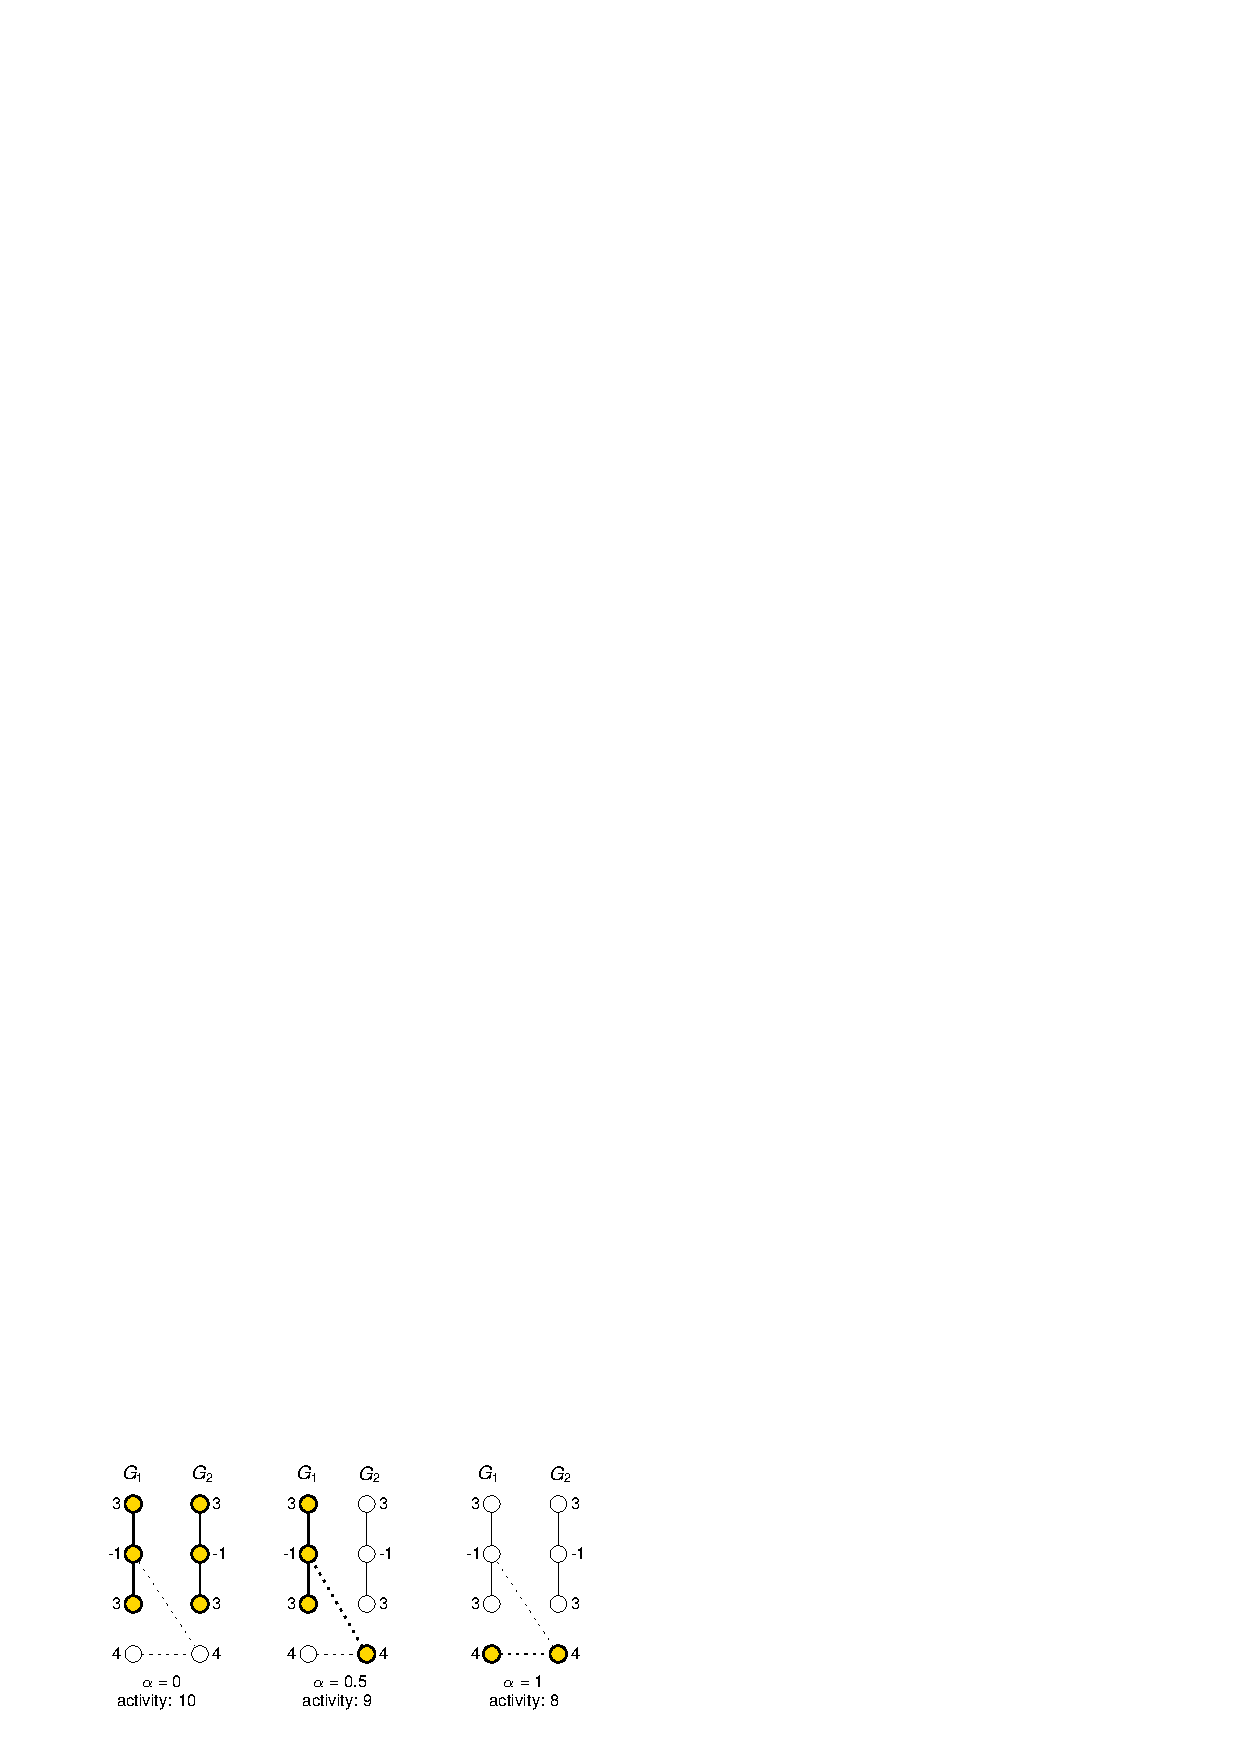
\includegraphics{exmpl_tradeoff_alpha}
			\caption[Trade-off between activity and conservation]{\textbf{Trade-off between activity and conservation.}
				Three optimal solutions (indicated in yellow) for varying conservation ratios $\alpha$ in a toy example instance.
				Node activities are given next to the nodes, conserved node pairs are linked by dotted lines.
				The activity of a conserved module is the sum of the activities of its comprising nodes.
				The parameter $\alpha$ denotes the minimum fraction of nodes in a solution that must be conserved, \ie{} connected by a dotted line.
			}
			\label{fig:exmpl_tradeoff_alpha}
		\end{figure}

	\subsection{Mixed-Integer Linear programming approach}

		We formulate the conserved active modules problem as an integer programming (IP) problem in the following way.
		\allowdisplaybreaks
		\begin{alignat}{3}
		\label{eq:obj}           \max\: & \sum_{v \in V_1 \cup V_2} w_v x_v \\
		\label{eq:m_u}  \text{s.t.}\:\: & m_u = \max_{uv \in R}{x_u x_v} & u \in V_1\\
		\label{eq:m_v}                  & m_v = \max_{vu \in R}{x_u x_v} & v \in V_2\\
		\label{eq:b}                    & \sum_{v \in V_1 \cup V_2} m_v \geq \alpha \sum_{v \in V_1 \cup V_2} x_v &\\
		\label{eq:con}                  & \text{$G_1[\mathbf{x}]$ and $G_2[\mathbf{x}]$ are connected}&\\
		\label{eq:vars}                 & x_v, m_v \in \{0, 1\} & v \in V_1 \cup V_2
		\end{alignat}


		This formulation satisfies the properties of activity, conservation and modularity.

		\paragraph{Activity.}\mbox{}\\
		Variables $\mathbf{x} \in \{0, 1\}^{V_1 \cup V_2}$ encode the presence of nodes in the solution, \ie, for all $v \in V_1 \cup V_2$ we want $x_v = 1$ if $v \in V^*$ and $x_v = 0$ otherwise.
		%\[
		%	x_v = \begin{cases}1 & \text{if } v \in V^*\text{,}\\
		%	                   0 & \text{otherwise.}\end{cases}
		%\]
		The objective function \eqref{eq:obj} uses these variables to express the activity of the solution, which we aim to maximize.

		\paragraph{Conservation.}\mbox{}\\
		Variables $\mathbf{m} \in \{0, 1\}^{V_1 \cup V_2}$ encode the presence of conserved nodes in the solution.
		Recall that a node $u \in V_1^*$ ($u \in V_2^*$) that is present in the solution is conserved if there is another node $v \in V_2^*$ ($v \in V_1^*$) in the solution such that the two nodes form a conserved node pair $uv \in R$ ($vu \in R$).
		This corresponds to constraints \eqref{eq:m_u} and \eqref{eq:m_v}.
		Indeed, constraints \eqref{eq:m_u} encode that a node $u \in V_1$ that is present in the solution ($x_u = 1$) is conserved if there exists a related node $v \in V_2$ ($uv \in R$) that is also present in the solution ($x_v = 1$).
		Similarly, constraints \eqref{eq:m_v} defines conserved nodes in $V_2$ that are present in the solution.
		We linearize $x_ux_v$, in a standard way, by introducing binary variables $\mathbf{z} \in \{0,1\}^R$ such that $z_{uv} = x_ux_v$ for all $uv \in R$:
		\allowdisplaybreaks
		\begin{alignat}{3}
		\label{eq:z1} & z_{uv} \leq x_u                 & uv \in R\\
		\label{eq:z2} & z_{uv} \leq x_v                 & uv \in R\\
		\label{eq:z3} & z_{uv} \geq x_u + x_v - 1 \quad & uv \in R\\
		\label{eq:vars2} & z_{uv} \in \{0,1\} & uv \in R
		\end{alignat}

		Subsequently, we model the max function in \eqref{eq:m_u} and \eqref{eq:m_v} as follows.
		\allowdisplaybreaks
		\begin{alignat}{3}
		\label{eq:m1}   & m_u \geq z_{uv}   & \forall v \in {V_2}^*\text{ st. }uv \in R\\
		\label{eq:m1b}  & m_v \geq z_{uv}   & \forall u \in {V_1}^*\text{ st. }uv \in R\\
		\label{eq:m2}   & m_u \leq \sum_{uv \in R}z_{uv}\quad  & u \in V_1\\
		\label{eq:m3}   & m_v \leq \sum_{uv \in R}z_{uv}  & v \in V_2
		\end{alignat}
		This set of constraints encode the two required conditions:
			\[
				m_u = \begin{cases}1 & \text{if at least one of its counterpart is present,}\\
				                   0 & \text{otherwise.}\end{cases}
			\]
		On one hand, \eqref{eq:m1} define a set of constraints: one for each node $v \in {V_2}^*$ such that $uv\in R$. This set of constraints effectively instruct the ILP that $m_u$ must be 1 if at least one of the counterparts of $u$ is in the solution.
		The same reasoning goes for \eqref{eq:m1b}.
		On the other hand, \eqref{eq:m2} constraint the variable $m_u$ to be 0 if none of the counterparts of $u$ are in the solution.
		The same reasoning goes for \eqref{eq:m3}.

		We model the required degree of conservation by constraint \eqref{eq:b}: the fraction of conserved nodes in the solution is at least $\alpha$.

		\paragraph{Modularity.}\mbox{}\\
		In addition, we satisfy the modularity property by requiring in \eqref{eq:con} that $G_1[\mathbf{x}]$ and $G_2[\mathbf{x}]$ are connected.

		Constraint \eqref{eq:con} states that the nodes encoded in the solution $\mathbf{x}$ induce a connected subgraph in both $G_1$ and $G_2$.
		There are many ways to model connectivity, \eg, using flows or cuts
		\parencite{magnanti1995optimal}.
		However, \textcite{dilkina2010solving} showed that cut-based formulations perform better in practice.
		Recently, \textcite{alvarez2013maximum} have introduced a cut-based formulation that only uses node variables.
		In an empirical study, the authors show that their formulation outperforms other cut-based formulations.
		We model connectivity along the same lines.
		Since the constraints that we will describe are similar for both graphs, we introduce them only for graph $G_1 = (V_1, E_1)$.
		\allowdisplaybreaks
		\begin{alignat}{3}
		\label{eq:sumy} & \sum_{v \in V_1} y_v \leq 1 & \\
		\label{eq:y}    & y_v \leq x_v & v \in V_1\\
		\label{eq:cut}  & x_v \leq \sum_{u \in \delta(S)} x_u + \sum_{u \in S} y_u
                  		\quad & v \in V_1, \{v\} \subseteq S \subseteq{V_1}\\
		\label{eq:vars3} & y_v \in \{0,1\} & v \in V_1 \cup V_2
		\end{alignat}
		Where $\delta(S) = \{ v \in V_1 \setminus S \mid \exists u \in S: uv \in E_1 \}$ denotes the \emph{neighbors} of $S$.

		The modularity property states that $\mathbf{x}$ should induce a connected subgraph in $G_1$.
		However in our model, we don't explicitely model graph connectevity, and model local connectivity instead.
		The first sum of \eqref{eq:cut} state that $x_v$ can only be $1$ if, for all sets $S \subseteq V$ containing $v$, it holds that there is a neighbor $u$ of $S$ in the solution.
		Informally, this constraint is a form of expension where we require the nodes in the solution to be part of the neighborhoud of the other nodes in the solution, hence forming a connected subgraph.
		However this is not sufficient, because this would require all nodes to be included in the end.
		We solve this by introducing binary variables $\mathbf{y} \in \{0, 1\}^{V_1}$ that determine a root node, which serves as a local expension termination condition.
		First, constraints \eqref{eq:sumy} and \eqref{eq:y} state that at most one node $v$ part of the solution can also be the root node -- in which case $y_v = 1$.
		Second, the last sum of \eqref{eq:cut} state that $x_v$ can only be $1$ if, for all sets $S
		\subseteq V$ containing $v$, it holds that the root node is in $S$.
		Informally and integrating the first sum, this constraint encode that the graph is locally connected around $v$ if, for all possible sets $S \subseteq V$ containing $v$, either the root node is part of $S$ or at least one node of the neighborhoud of $S$ is part of the solution.

		There is an exponential number of such constraints.
		Therefore, we cannot add all them to our initial formulation.
		Instead we use a branch-and-cut approach, that is, at every node of the branch-and-bound tree we identify all violated constraints and add them to the formulation.
		Finding violated inequalities corresponds to solving a minimum cut problem, which we do using the algorithm by \textcite{boykov2004experimental}.

		%In the separation, we also generate back cuts and nested cuts.
		%Details are omitted due to space limitation.

		\paragraph{}
		To further improve the performance, we also strengthen our model with the following constraints. None of those constraints are necessary, but they help the ILP solver by reducing the search space.
		\begin{alignat}{3}
		\label{eq:y2}   & y_v = 0 & v \in V, w_v < 0\\
		\label{eq:sumy2} & \sum_{u \in V} y_u \geq x_v & v \in V, w_v\geq 0\\
		\label{eq:1neighbor} & x_v \leq \sum_{u \in \delta(\{v\})} x_u + y_v \quad & v \in V\\
		\label{eq:sym_break} & y_v \leq 1 - x_u \quad & u, v \in V, u < v, w_u \geq 0, w_v \geq 0
		\end{alignat}
		Constraints \eqref{eq:y2} states that the root node must be a positively weighted node, which reduces the search space of the root node.
		Constraints \eqref{eq:sumy2} explicitly state that the root node variable must be 1 if at lease one of the positive nodes is in the solution.
		This was already required for the previous set of constraints but never explicitly instructed to the solver.
		Constraints \eqref{eq:1neighbor} is an optimization for the cases where the set $S$ in \eqref{eq:cut} is a singleton.
		Finally, constraints \eqref{eq:sym_break} are symmetry breaking constraints: they encore an ordering for the possible root selections.
		It effectively requires that among all positively weighted nodes in the solution, the root node is the smallest one -- according to some arbitrary order\footnote{In our case: the order of apperances of the nodes in the network definition.}.
		This last set of constraints also provide determinism: the ordering garantee that two runs of the ILP will choose the same root node.

\section{Material and methods}
\label{sec:xexp}

We apply our method to the recently discovered interleukin-17 producing helper T~cells (Th17), which exposes the problems highlighted in \cref{sec:xhintro}.

These cells form a separate subset of helper T~cells with a differentiation pathway distinct from those of the established Th1 and Th2 cells \parencite{park2005distinct}.
Th17 cells are known to contribute to pathogenesis of inflammatory and autoimmune diseases such as
asthma, rheumatoid arthritis, psoriasis and multiple sclerosis and play also a role in cancer immunology \parencite{wilke2011deciphering}.
They originate from na\"ive helper cells, responding to environmental stimulus by activating a differentiation and specialization process \parencite{steinman2007brief}.

Understanding the pathways and regulatory mechanisms that mediate the decision making processes resulting in the formation of Th17 is a critical step in the development of novel therapeutics that will facilitate rational manipulation of the immune response.
Unfortunately, the vast majority of data collected so far originates from studies performed on mice \parencite{tuomela2012identification} and, most importantly, a comprehensive comparison of the Th17 differentiation process in model organisms and in human is missing.
Several studies indicate that the differentiation and phenotype of human and mouse Th17 cells are similar \parencite{annunziato2009studies}.
Both subsets serve similar pro-inflammatory functions and produce the same hallmark cytokines and similar receptors.
Furthermore, most of the already identified regulator genes show high sequence conservation.

These findings indicate that the differentiation process seems well conserved between human and mouse and that a cross-species approach is reasonable.
Other studies, however, show stimulus requirements for effective differentiation of human cells that differ from those required for mice \parencites{mcgeachy2008th17}{o2008differentiation}{annunziato2009human}.

The simultaneous analysis of both human and mouse expression data allows the identification of conserved candidate regulators% that are likely to be key regulators of the differentiation process
, as well as potential drug targets.
Most of our current understanding on Th17 cell differentiation relies on studies carried out in mice, whereas the molecular mechanisms controlling human Th17 cell differentiation are less well defined.
A characterization of the similarities and differences will not only increase our understanding of this fundamental process, but is also essential for sound translational research.

	\subsection{Experimental procedure}

% In \citet{Tuomela:2013ly}, RNA-Seq samples of both human and mouse CD4+ cells
	% were polarized toward Th17 direction and we summarize here their
	% experimental procedure. Human CD4+ cells were obtained from  mononuclear
	% cells purified from the umbilical cord blood of healthy neonates. Cells
	% from several individuals were pooled, then activated using anti-CD3 and
	% anti-CD28. Th17 differentiating cytokines consisted of IL6, IL1B and TGFB,
	% along with neutralizing anti-IFNG and anti-IL4. Cells that were activated
	% without Th17 cytokines were cultured as controls (Th0). Mouse CD4+ cells
	% were obtained from C57BL/6 mice bred under specific conditions devoid of
	% pathogens. Similarly to human cells, mouse CD4+ cells were activated
	% (anti-CD3 and anti-CD28), polarized (TGFB, IL6, IL1B) and control mouse
	% cells (Th0) were also cultured. Three biological replicates of mouse and
	% human cells, for both conditions, were collected at \unit{0}5]{h},
	% \unit{1}{h}, \unit{2}{h}, \unit{4}{h}, \unit{6}{h}, \unit{12}{h},
	% \unit{24}{h}, \unit{48}{h}, \unit{72}{h} time points. Following
	% manufacturer instructions, RNA was isolated and DNase treated before being
	% sequenced (50nt reads) on a HiSeq \comment[Daniela]{Do we know the HiSeq
	% version? 1000, 2000, 2500?} instrument. Base calling and quality control
	% was performed using CASAVA 1.8.

We summarize here the experimental procedure followed by \textcite{tuomela2012identification} and \textcite{yosef2013dynamic} to generate transcriptomic profiles.

\textcite{tuomela2012identification} isolated CD4+ T-cells from umbilical cord blood of several healthy neonates, arranged in three different pools, then activated with anti-CD3 and anti-CD28.
Cells from each pool were then divided in two batches, one to be polarized toward Th17 direction, and one serving as control (Th0).
Th17 differentiating cytokines consisted of IL6~(\unit{20}{\nano\gram\per\milli\liter}), IL1B~(\unit{10}{\nano\gram\per\milli\liter}) and TGFB~(\unit{10}{\nano\gram\per\milli\liter}), along with neutralizing anti-IFNG~(\unit{1}{\micro\gram\per\milli\liter}) and anti-IL4~(\unit{1}{\micro\gram\per\milli\liter}).
%Cells that were activated without Th17 cytokines were cultured as controls (Th0).
Three biological replicates of human cells, for both conditions (coming from each pool), were collected between \unit{0.5-72}{h} (\unit{0.5}{h}, \unit{1}{h}, \unit{2}{h}, \unit{4}{h}, \unit{6}{h}, \unit{12}{h}, \unit{24}{h}, \unit{48}{h}, \unit{72}{h} time points) and hybridized on Illumina Sentrix HumanHT-12 Expression BeadChip Version~3.
The microarray data were analyzed using the beadarray Bioconductor package \parencite{dunning2007beadarray}.

\textcite{yosef2013dynamic} purified CD4+ T-cells from spleen and lymph nodes from wild type C57BL/6 mice, then activated with anti-CD3 and anti-CD28. For Th17 differentiation, cells were cultured with TGFB (\unit{2}{\nano\gram\per\milli\liter}), IL6 (\unit{20}{\nano\gram\per\milli\liter}), IL23 (\unit{20}{\nano\gram\per\milli\liter}) and IL1B (\unit{20}{\nano\gram\per\milli\liter}) during \unit{0.5-72}{h} (at time points \unit{0.5}{h}, \unit{1}{h}, \unit{2}{h}, \unit{4}{h}, \unit{6}{h}, \unit{8}{h}, \unit{10}{h}, \unit{12}{h}, \unit{16}{h}, \unit{20}{h}, \unit{24}{h}, \unit{30}{h}, \unit{42}{h}, \unit{48}{h}, \unit{50}{h}, \unit{52}{h}, \unit{60}{h}, \unit{72}{h}), and finally hybridized on an Affymetrix HT\_MG-430A.
%Highly-correlated replicates were generated for 8 time points (\unit{1}{h}, \unit{4}{h}, \unit{10}{h}, \unit{20}{h}, \unit{30}{h}, \unit{42}{h}, \unit{52}{h}, \unit{60}{h}).


\subsection{Microarray processing, statistical analysis and node scoring}
\label{sub:statistical_analysis_and_node_scoring}
% Sequence reads were mapped using TopHat 1.3.2 to the GRCh37 release 63 human
% genome and to the NCBIM37 release 63 mouse genome. Gene-wide read counts for
% Ensembl genes were estimated using HTSeq 0.5.4p5, discarding reads overlapping
% multiple genes. Differential expression between Th17 and Th0 conditions was
% estimated using the edgeR package \citep{Robinson:2010ve}.

% For each species, differential expression calling was performed at each time point independently.
% For the human samples, samples were indicated as paired according to the
% experimental design so as to account for the pooled human samples. For mouse
% samples, calling was performed on all Th0 vs Th17 samples, regardless of the
% mouse donor. In both cases, dispersion was estimated as gene-wise dispersion.


Preprocessed and quantile normalized data sets were downloaded from GEO under the accession numbers GSE43955 and GSE35103.
As downloaded from GEO, both the human and the mouse time-series were already filtered by retaining only the probes with detection p-values $< 0.05$ in at least one time point and one condition.
Following the original studies, we further only retained probes having a standard deviation $> 0.15$ over all the conditions and time points; as well as being annotated by a single Ensembl gene.
Finally, a single probe was selected for each gene by taking, for each Ensembl gene, the probe having the largest variance accross all samples.
In total, 12,307 and 18,497 probes passed the filters for the mouse and human data set, respectively.

Differential expression between Th17 and Th0 conditions were estimated using the limma package \parencite{smyth2005limma}.
Human samples were indicated as paired according to the experimental design so as to account for the pooled human samples.
For mouse samples, calling was performed on all Th0 vs Th17 samples, regardless of the mouse donor.
To determine which genes were differentially expressed at a given time point, we used a linear model to estimate the interaction between the treatment and the time effect.
The linear models used for the human and mouse studies include one interaction term for each time point and exclude the intercept (In R, the formula reads: $\mathrm{\sim 0+treat:time}$).
% \textcolor{red}{The linear models used in each of the human and mouse studies are defined as $\mathrm{\sim 0+treat:time}$, interpreted as 1) no intercept term and 2) one interaction term for each time point (R formula syntax).
Differential expression at any time point $K$ of interest were determined by the contrasts $\mathrm{Th17.time_{K} - Th0.time_{K}}$.
We report in this study results for the following time points: \unit{2}{h}, \unit{4}{h}, \unit{24}{h}, \unit{48}{h}, \unit{72}{h}.

%To deal with the lack of replicates in the highly variable late time points of
%the mouse data (\unit{2}{h}, \unit{24}{h}, \unit{48}{h}, \unit{72}{h}), we
%relied on the neighboring time point to estimate the
%treatment effect in this time frame by performing a weighted regression. For
%example, identification of differential expression at \unit{48}{h} is made by
%estimating the effect $8/10 \cdot Th17 : time_{48} + 1/20 \cdot Th17 : time_{42}
%+ 3/20 \cdot Th17:time_{50}$.


%%%% Old probe selection procedure 
% Once differential expression was tested for at the probe-level, we
% summarized the results at the gene-level by taking the smallest
% p-value of any probe capturing a transcript of that gene. 
\noindent\paragraph{}\noindent Following \parencite{dittrich2008identifying}, we computed positive and negative scores for each gene at each time point by fitting a beta-uniform mixture model using the implementation in the BioNet package \parencite{beisser2010bionet}.
The method proceeds as follows:

Similarly to \parencite{pounds2003estimating}, the distribution of the gene-wise p-values $x = x_1, \ldots, x_n$ is described as a beta-uniform mixture (BUM) model, which is a mixture of a $B(a, 1)$ beta distribution (signal) and a uniform distribution (noise):   % By definition the
% p-value is uniformly distributed under the null hypothesis
% (noise).
% the combined
% distribution of signal and noise p-values can empirically be modelled
% by a beta-uniform mixture (BUM) model, where the signal component is modeled by a beta distribution $\Beta(a,1)$ and the noise component is modeled by a uniform distribution:
% The $\Beta(a,b)$ distribution is given by
% \begin{eqnarray*}
%    f(x) & = & \frac{\Gamma(a+b)}{\Gamma(a)\Gamma(b)}\;x^{a-1}(1-x)^{b-1},
% \end{eqnarray*}
% where $\Gamma(\cdot)$ denotes the Gamma function.
% The distribution of the derived p-values reduces to
$\lambda + (1- \lambda)ax^{a-1}$, for $0 < a < 1$, with mixture parameter  $\lambda$ and shape parameter $a$ of the beta distribution.
The log likelihood is defined as $\log\left(\lambda, a;x\right) = \sum_{i=1}^{n}\log(\lambda+(1-\lambda)a x_i^{a-1})$, and consequently the maximum-likelihood estimations of the unknown parameters are given by $[\hat{\lambda}, \hat{a}] = \argmax_{\lambda,a} \left(\lambda,a;x\right)$.
%%\begin{equation*}
%   . %%\enspace.
%%\end{equation*}
The parameter estimates have been obtained using numerical
optimization. % Based on the fitted mixture model the distribution of
% p-values can be decomposed into a signal and a noise component, from
% which the node score is calculated as a log likelihood ratio of the signal and the noise component.
% Similar to classical hypothesis tests, a threshold value that
% discriminates signal from noise can be introduced.
As detailed in \parencite{pounds2003estimating}, the BUM model allows the estimation of a false discovery rate ($\FDR$) that can be controlled via a p-value threshold $\tau(\FDR)$.
The adjusted log likelihood ratio score is then defined as
\[
% \begin{eqnarray}
%    S^{\FDR}(x)  = \log\left(\frac{\Beta(a,1)(x)}{\Beta(\tau^{\FDR},1)(x)\Beta(1,1)(x)}\right) =   \log\left(\frac{a x^{a-1}}{a \tau^{a-1}}\right) = (a-1)\left(\log(x) - \log(\tau(\FDR))\right),
s(x, \FDR) =   \log\frac{\hat{a} x^{\hat{a}-1}}{\hat{a} \tau(\FDR)^{\hat{a}-1}}
= (\hat{a}-1)\left(\log(x) - \log(\tau(\FDR))\right)\:.
\label{eqn:scoreFDR}
\]
%The adjusted and unadjusted scores only differ by an additive offset
%which is dependent on the parameter $\tau_{\FDR}$ and can be regarded
%as a significance threshold. Thus, 

Genes whose differential expression is considered significant given the FDR threshold obtain a positive score while genes showing no differential expression will receive a negative score. % It can easily be seen that for $\tau(\FDR) \rightarrow 0 $ the score $s(x) \rightarrow -\infty$ and for $\tau(\FDR) \rightarrow 1$ all scores will be positive and the $\FDR$ will be equal to $\lambda$, the mixture parameter of the noise model.
The size of the resulting module can be regulated with this FDR parameter.
Throughout this study, $\FDR=0.1$ was used for all samples and species.

However, due to the experimental noise and paired design, the human samples have much higher intra-group variance, resulting in significant calls having p-values orders of magnitude higher than the mouse calls.
This results in a range of scores that is much narrower for human than for mouse, possibly imbalancing results towards mouse modules.
To correct for this effect, scores of mouse genes were rank normalized to the scores of the human genes as follows: the scores (as defined by the BUM model) were sorted, and for each gene the score of the $i$-th mouse gene was set to the score of the $i$-th human gene.

Comparison of the distribution of scores before and after normalization showed that compared to usual Benjamini-Hochberg FDR and log fold change cut-offs ($\absLOGFC \geq 1)$, the loss in statistical power was inconsequential and that this procedure ensured that mouse and human genes had comparable score distributions.

% In the following, all reported FDRs were obtained using the Benjamini-Hochberg procedure.
%Finally, only genes coding for a protein present in the STRING network (see Sect.~\ref{sub:public_datasets}) were kept. % Table \ref{table:calls} summarizes the number of differentially expressed genes called at each time point for the two species.


% \begin{table*}[ht]
% \label{table:calls}
% \centering
% \begin{tabular}{r|l|ll || lrrrrr}
% \multirow{2}{*}{Species} & \multicolumn{3}{c||}{Gene characteristic} &  \multicolumn{5}{c}{Time} \\
% \cline{2-9}
%  ~ & BUM score & $FDR\leq 0.01$ & $abs(LogFC) \geq 1.0$ & 2h & 4h & 24h & 48h & 72h \\
% \hline
% \hline
% %  \cline{2-9}
%  \multirow{6}{*}{Human} & \multirow{2}{*}{Negative} & False & False & 8355 & 8424 & 8346 & 8282 & 8189 \\
%   ~ & ~ & False & True &  17 &  23 &  26 &  22 &  19 \\
%   \cline{2-9}
%   ~ & \multirow{4}{*}{Positive} & False & False &   4 & 0 &   4 &  10 &  65 \\
%   ~ & ~ & False & True &   2 & 0 & 0 &   1 &   2 \\
%   \cline{3-9}
%   ~ & ~ & True & False &  37 &   2 &  39 &  75 & 99 \\
%   ~ & ~ & True & True &  38 &   4 &  38 &  63 &  79 \\
%   \hline
%   \hline
%   \multirow{6}{*}{Mouse} & \multirow{4}{*}{Negative} & False & False & 6569 & 6655 & 6422 & 6146 & 5542 \\
%   ~ & ~ & False & True &  59 &  17 & 73 &  25 & 38 \\
%   \cline{3-9}
%   ~ & ~ & True & False & 115 & 108 & 106 & 405 & 790 \\
%   ~ & ~ & True & True & 98 &  65 & 163 & 204 & 343 \\
%   \cline{2-9}
%   ~ & \multirow{2}{*}{Positive} & True & False & 11 &   1 & 2 &   5 & 4 \\
%   ~ & ~ & True & True &  52 &   7 &  62 & 124 & 201 \\
%    \hline
% \end{tabular}
% \caption{Contingency table summarizing the characteristics of the nodes used as input to \xHeinz for the identification of conserved Human and Mouse modules during Th17 differentiation. In this setup, \xHeinz received as input two species-specific STRING network, a mapping between Human and Mouse proteins based on ENSEMBL orthology, and a mapping from protein to a real-valued Beta-Uniform (BUM) score. Each cell in this table reports the number of genes coding for a protein from the species-specific STRING network, for each of the 5 instances (2h--72h), for each species, and satisfying any conjunction of these three properties: 1)~\textbf{BUM score:}~being scored positively using a rank-normalized BUM decomposition of the distribution of the p-values of differential expression between Th17 and Th0 conditions (limma moderated t-test); 2)~\textbf{FDR:}~having a Benjamini-Hochberg FDR below $\tau\leq0.01$ under the same hypothesis and 3)~\textbf{logFC:}~having an absolute log-fold change $\geq 1$. Rows containing only zeros are omitted. Details are provided in section \ref{sub:statistical_analysis_and_node_scoring}.}
% \end{table*}
% \comment{Consider increasing the logFC threshold to 1.5 or 2}

\subsection{Network and orthology databases}
\label{sub:public_datasets}

The human and mouse background networks were downloaded from STRING v9.1, protein.actions.detailed.v9.1.txt \parencite{franceschini2013string}, which is a database that contains experimentally verified direct protein interactions.
Note that this network also contains interactions predicted based on orthology, so-called \emph{interologs}.
Ideally, we would prefer to use only experimentally predicted interactions, but currently, for mouse, such available data is too incomplete to result in a meaningful background network.
Outlier nodes with a degree above $40$ times the interquartile range plus the 75th percentile of the distribution of all node degrees were removed (ELAVL1, UBC, Ubb, Ubc).
The resulting mouse network has $16,821$ nodes and $483,532$ edges and the human network has $16,255$ nodes and $315,442$ edges.


For any given timepoint, we performed a preprocessing step where we retained the subgraphs of the input networks induced by the genes that meet the microarray filtering criteria.
This reduced the number of nodes to 8,453 human nodes, 6,882 mouse nodes and 14,779 nodes in the orthology mapping.
Among these, up to 250 nodes (depending on the time point) have positive scores.
The rank normalization as described in \cref{sub:statistical_analysis_and_node_scoring} ensured that the number of positive human nodes is in the order of the number of positive mouse nodes.

Orthology information was downloaded from Ensembl release 59 \parencite{flicek2013ensembl} and all human and mouse orthologs were kept, regardless of the identity scores.
The orthology mapping corresponds to a bipartite graph involving $67,304$ human proteins and $43,953$ mouse proteins linked by $104,007$ edges, grouped in $16,552$ bicliques with an average size of $6.72$ proteins (SD: $5.34$).

	\subsection{Results}

		\subsubsection{\xheinz{} identifies statistically significant conserved modules at different levels of conservation}
		\label{sec:xheinz-effic-ident}

			We applied \xheinz{} on samples from the Th17 human and mouse data sets for time points \unit{2}{h}, \unit{4}{h}, \unit{24}{h}, \unit{48}{h} and \unit{72}{h}.
			We solved these instances for different values of $\alpha \in [0, 1]$ with a step size of $0.1$.
			All computations were done in single-thread mode on a desktop computer (Intel XEON e5 3~Ghz) with 16~Gb of RAM and a time limit of 12,000 CPU seconds.
			After this timeout, the best feasible solution is returned by the solver.

			\Cref{fig:scores} shows for the five time points and eleven values of the $\alpha$ parameter, the human and mouse scores of the found modules as well as the distribution of the module contents.
			For 26 of the 55 instances we solved the conserved active modules problem to provable optimality  within the time and memory limit.
			The optimality gap of a solution is defined as $(\mathit{UB} - \mathit{LB}) / \abs{\mathit{LB}}$, where $\mathit{LB}$ and $\mathit{UB}$ are the value of the best solution and the lowest upper bound as identified by the branch-and-cut algorithm, respectively.
			Of the 29 instances that are not solved to optimality, 22 have a gap smaller than $5\%$.

\begin{figure}[btp]
  \centering
  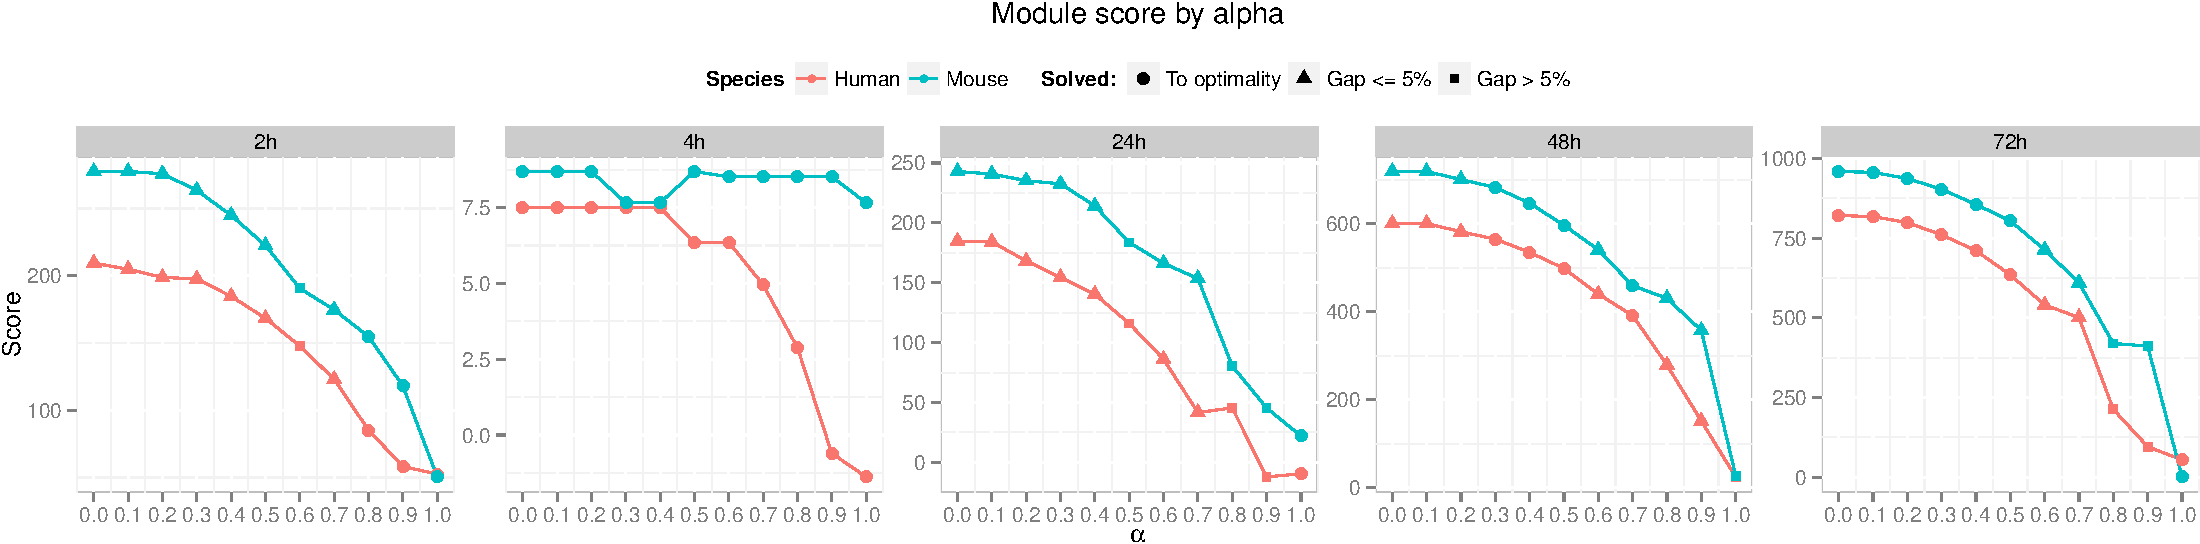
\includegraphics[width=\linewidth,trim=0 0 0 10mm,clip]{img/score_by_alpha_array-crop.pdf}\\
  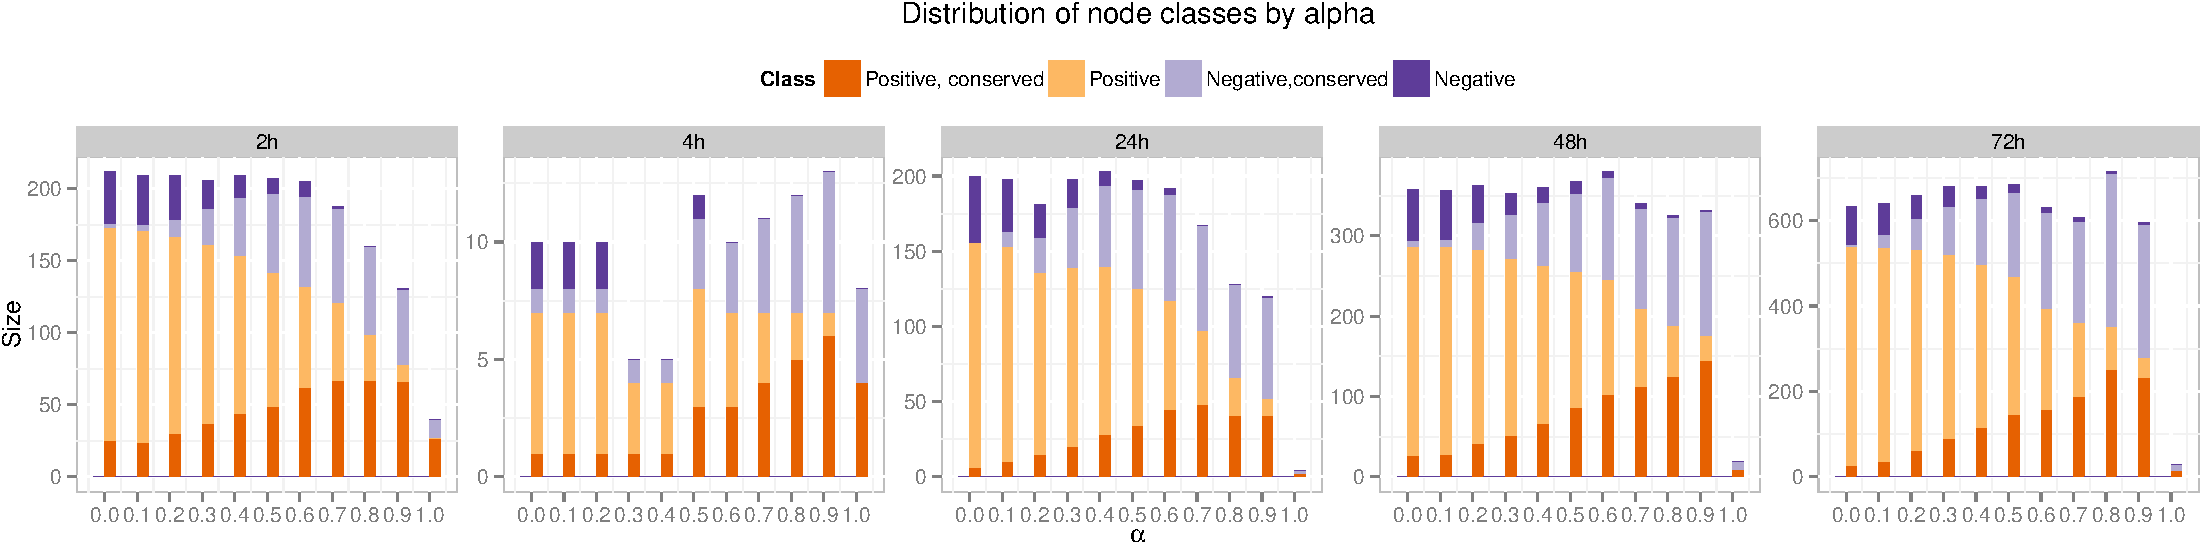
\includegraphics[width=\linewidth,trim=0 0 0 10mm,clip]{img/node_classes_by_alpha_array_scores-crop.pdf}
  \caption[Statistics of \xheinz{} solutions]{\textbf{Statistics of \xheinz{} solutions.}
  	  The conserved active module problem was solved for five time points (columns) over a sequence of 11 consecutive values of the $\alpha$ conservation parameter ($x$-axis).
  	  We report in the top row the score of the best solution ($y$-axis) and whether optimality was proven by our algorithm (circles).
  All runs were limited to 12,000 CPU seconds on a standard desktop computer.
  The second row illustrates how module contents vary as $\alpha$ increases.
  The height of each bar indicates the size of the respective module, colors indicate the fraction of positive and conserved nodes.
  \label{fig:scores}}
\end{figure}

Any feasible solution for a conservation ratio of $\alpha$ is also a solution for any $\alpha' \leq \alpha$.
We indeed see in \cref{fig:scores} that this property holds, the solution values decrease monotonically with increasing $\alpha$.
Consequently, if we obtain an optimal solution (\ie, with maximal activity score) for $\alpha'$ then, any solution for $\alpha$ must have its activity score that is greater or equal to the one for $\alpha'$.
When we only account for the optimal solutions of our instances, we indeed see that this property holds.
% MEK: I DON'T UNDERSTAND THIS THE FOLLOWING
%Conversely, this implies that we can bound the optimal activity scores whenever
%we obtain optimal solutions for neighboring $\alpha$ parameter values; and thus that
%several of our solutions were close to the real optimum. 
% HS: Mohammed, as an example, take 48h 0.5 and 0.8, both are solved to optimality. This imply that the score of the optimal solutions for 0.6 and 0.7 are within the scores of the 0.5 and the 0.8, and since our suboptimal solutions are within this range, this means that we not so far from them. 

As an added validation, we observe that the solutions for $\alpha=0$ (no conservation constraints) are identical to the solutions obtained by running the single species method Heinz, described by \textcite{dittrich2008identifying}, separately on the two networks.

There is a sharp decrease in module size for $\alpha = 1$.
Indeed, this is the most restrictive setting since it enforces that all the nodes in a module must be conserved.
We also observe that as $\alpha$ increases, both positive and negative \emph{conserved} nodes are added, indicating that we manage to retrieve informative nodes in a gradual manner.
See also \cref{app:significance} for a detailed analysis of module overlap for all combinations of $\alpha$ values.

When we compare solutions across time points, we see that the conserved active modules capture two phases of the differentiation process.
We observe high activity at \unit{2}{h} as well as at the late time points.
Several authors reported such biphasic behavior during early Th17 differentiation, for example \textcites{ciofani2012validated}{yosef2013dynamic} in mouse, and \textcite{tuomela2012identification} for human.
The low activity score observed at the \unit{4}{h} time point is in line with \textcite{yosef2013dynamic}'s mouse studies, which suggest that after the initial induction sustained by Stat3 and Stat1 in the first four hours, a phase of Rorc induction takes place and lasts until the \unit{20}{h} time point, after which the effective protein level of Rorc starts to increase and to trigger the cytokine production phase.
Our model and the solutions obtained suggest that these dynamics are conserved between the two organisms.

Furthermore, \cref{fig:spider-xheinz_modules} illustrates the strong conservation of these overall dynamics, in human and mouse at \unit{2}{h}.
The plots show that in our modules all but two conserved gene pairs change expression in the same direction.
It is worth noting that we do not enforce any conservation of directionality in the \xheinz{} model.

\begin{landscape}
\begin{figure}[h]
  \centering
  %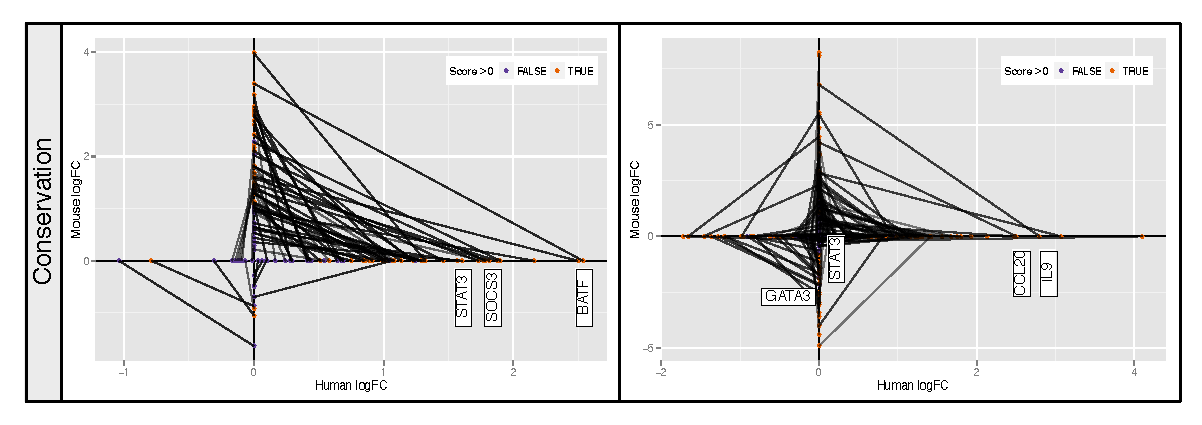
\includegraphics[width=1\linewidth]{spider_panel.pdf}
  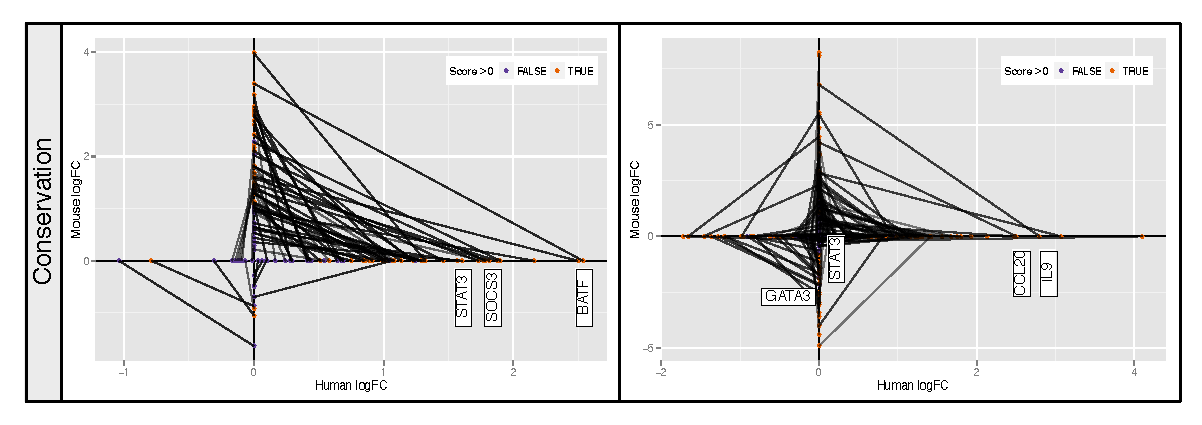
\includegraphics{spider_panel.pdf}
  \caption[Comparison of log fold change expression in mouse and human for conserved gene pairs at \unit{2}{h} and \unit{48}{h}]{\textbf{Comparison of log fold change expression in mouse and human for conserved gene pairs at \unit{2}{h} (left) and \unit{48}{h} (right).}
 Each panel shows the log fold change correlation between conserved gene pairs:
 For each pair, a line segments connects the human logFC ($x$-axis) to the mouse
 logFC ($y$-axis). Point color indicates whether the human or mouse gene has a
 positive score.
      A line segment in the 1st or 3rd quadrant
   signifies positively correlated logFC values whereas a link in the
   2nd and 4th quadrant corresponds to negative correlation. The sign
   of the activity score is indicated by the coloring. Genes discussed
   in the main text are indicated with white boxes.}
  \label{fig:spider-xheinz_modules}
\end{figure}
\end{landscape}


\subsubsection{Early regulation of Th17 differentiation is conserved between human and mouse}
\label{sub:main_regulation_of_th17_differentiation_is_conserved_between_human_and_mouse}

In the following, we study the two phases of the Th17 differentiation process in more detail.
We focus on the \unit{2}{h} and \unit{48}{h} time points.
We selected for this evaluation $\alpha=0.8$ for both time points, as this value provides a balance between conservation and activity and produces modules of interpretable size.
All results at all time points are available on the accompanying website.
\Cref{fig:panel_wht-xheinz_modules} reports a reduced version of the resulting human and mouse Th17 modules for the two time points, and \cref{fig:full_1} and \cref{fig:full_2} show the full, unfiltered module contents of the modules.

We assess statistical significance of the resulting modules by performing 100 runs on randomized networks for each value of $\alpha$, and additional 400 runs for the selected $\alpha=0.8$.
We do this using two randomization methods: (1) permuting the node weights while keeping the graph fixed, and (2) permuting the network topology while keeping the node weights and the node degrees fixed as described in \parencite{mihail2003markov}.
With the exception of a few extreme cases at the \unit{48}{h} time point, all modules were found to be highly significant.
For details see \cref{app:significance}.

Our model for conserved modules relies on the hypothesis that similar biological processes between two related species are realized by orthologous genes.
To evaluate the relevance of the conserved modules returned by \xheinz, we solved the conserved active modules problem between the Th0 and Th17 conditions at \unit{2}{h} and \unit{48}{h}.

At the \unit{2}{h} time point, \xheinz{} identifies a conserved module consisting of $58$ human and $50$ mouse proteins.
Interestingly, both the human and mouse modules are centered around STAT3/Stat3, even if these genes are not the ones showing the higher fold change in both species.
STAT3 is a signal transducer having transcription factor activity and was shown to play a key role in the differentiation process of Th17 \parencite{harris2007cutting}.
Once activated by Th17 polarizing cytokines (such as IL6 in our case), it eventually binds to the promoter regions of IL17A/Il17a and IL17F/Il17f cytokines and activates transcription.
These cytokines are the hallmark cytokines produced by activated Th17 cells.
It is worth noting that IL17/Il17 cytokines and associated receptors are not in the \unit{2}{h} modules, as these proteins have been shown to be expressed only at later time points \parencite{tuomela2012identification}.
Moreover, STAT1/Stat1, another member of the STAT family, is part of the solution and belongs to the central core of the human and mouse modules, which is consistent with its major role during the early phases of Th17 differentiation \parencite{yosef2013dynamic}.


%%Il17a vs IL17F 
%We also observe that the STAT3/BATF/IL6ST/SOCS3 region of the \unit{2}{h} module is well-conserved.
%NOTCH1 has been recently implicated as an intrinsic requirement for Th17 polarization both in human and mouse.
%NOTCH1 directly targets the IL17 and RORC loci and its deficiency is associated with impaired Th17 differentiation~\parencite{keerthivasan2011notch}.
%We further expected that NOTCH1 is implicated in the early phase of the differentiation process as it directly activates transcription of these two Th17 hallmarks proteins that are expressed later.
%Similarly, Batf has been shown to directly control Th17 differentiation in mouse~\parencite{schraml2009ap} and BATF proteins are detected as early as after \unit{12}{h} of polarization in human~\parencite{tuomela2012identification}. 
%Similarly, SOCS3 is a known IL6 and IL21-induced negative regulator of Th17 polarization, that is eventually down-regulated by TGFB and IL6ST at a later phase in order to prolong STAT3 activation \parencites{zhu2008socs3,qin2009tgf}.
%
%Overall, these modules show highly conserved and significant enrichment for response to cytokine stimulus (Benjamini-Hochberg (BH) FDR 5.6e-4), JAK-STAT (BH FDR 4.8e-4) cascade and transcription regulator activity (BH FDR 2.3e-4), computed using the DAVID functional annotation chart \parencite{huang2008systematic}.
%This indicates that the identified module matches expected biological mechanisms observed at early phases~\parencite{ciofani2012validated}.
%Furthermore, comparison of the dynamics of expression shows that genes differentially expressed in both species change expression in the same direction (see Supplementary~Text~A.3).

%\comment[Hayssam]{Add IL2RB/CXCR5 details? Add SOCS3 role. STAT1, easily
%involved. STAT1 implicated in the early phase, STAT3 in all phases [ciofiani]}

We also applied \xheinz{} to find a conserved module at a later time point (\unit{48}{h}).
Kinetics analysis of Th17 differentiation showed that the effective secretion of Th17 hallmark cytokines only happens after several days of polarization \parencites{tuomela2012identification,yosef2013dynamic} and we do observe in these modules a significant enrichment for interleukin related proteins present in both species, which was absent for the \unit{2}{h} modules, such as up-regulation of IL9/Il9.
Secretion of IL9 by Th17 cells have been demonstrated both in mouse and human cells \parencite{beriou2010tgf}, Il9 is known to be induced by Bcl3 \parencite{richard1999interleukin}, and Bcl3 inhibition has been recently shown to affect the function of Th17 cells in mouse \parencite{ruan2010roles}.
We also observe the conserved down-regulation of GATA3/Gata3, which is known to be the master regulator of Th2 cells \parencite{zheng1997transcription}, and is likely to constrain the Th17 regulation program \parencite{van2008enforced}.
Similarly to the modules found at \unit{2}{h}, the \unit{48}{h} modules are centered around STAT3, although at the \unit{48}{h} time point this gene is not differentially expressed anymore neither in human or mouse (resp.\ logFC of 0.17, score of -4.59 for human, and logFC 0.52, score of -3.21 for mouse).
This observation is in line with the major role of STAT3 along the differentiation process at all time points \parencite{yosef2013dynamic}.
To the contrary, STAT1 has been indicated as an exclusively early regulator \parencite{yosef2013dynamic} in mouse and is indeed not present anymore in the \unit{48}{h} modules.%, even though Stat1 is called as differentially expressed in the mouse measurements (BH FDR of $2e-04$, score of $-3.16$ for mouse; BH FDR of $0.99$, score of $-6.54$ for human).
%This demonstrates the strength of performing module identification in both species simultaneously in our setup.
%\comment[Hayssam]{Find ref about plasticity in the early tp. Compute overlap between early and late?}
% , the lack of evidence for differential expression in mouse (FDR 0.93) as well as the conservation constraint in the \xheinz formulation 

We also observe the presence of the RORA/RORC/Rora/Rorc members of the RORs family of intracellular transcription factors, which are considered to be the master regulators of the Th17 lineage \parencite{yang2008t}, and have been implicated in both species \parencite{crome2009role}.
Interestingly, these regulators are linked to the up-regulation of the vitamin-D receptor (VDR/Vdr), whose role in Th17 differentiation and several human auto-immune related disease have been recently studied \parencite{chang2010vitamin}.

\paragraph{}
In summary, our findings show the relevance of the identified conserved active modules with regard to the biological process of interest.
By requiring the active modules to contain a certain fraction of conserved nodes, \xheinz{} identifies the main core proteins involved in the differentiation of Th17.
Our analysis confirms that these proteins are very likely to have similar roles in both species.

\begin{figure}[t]
  \centering
  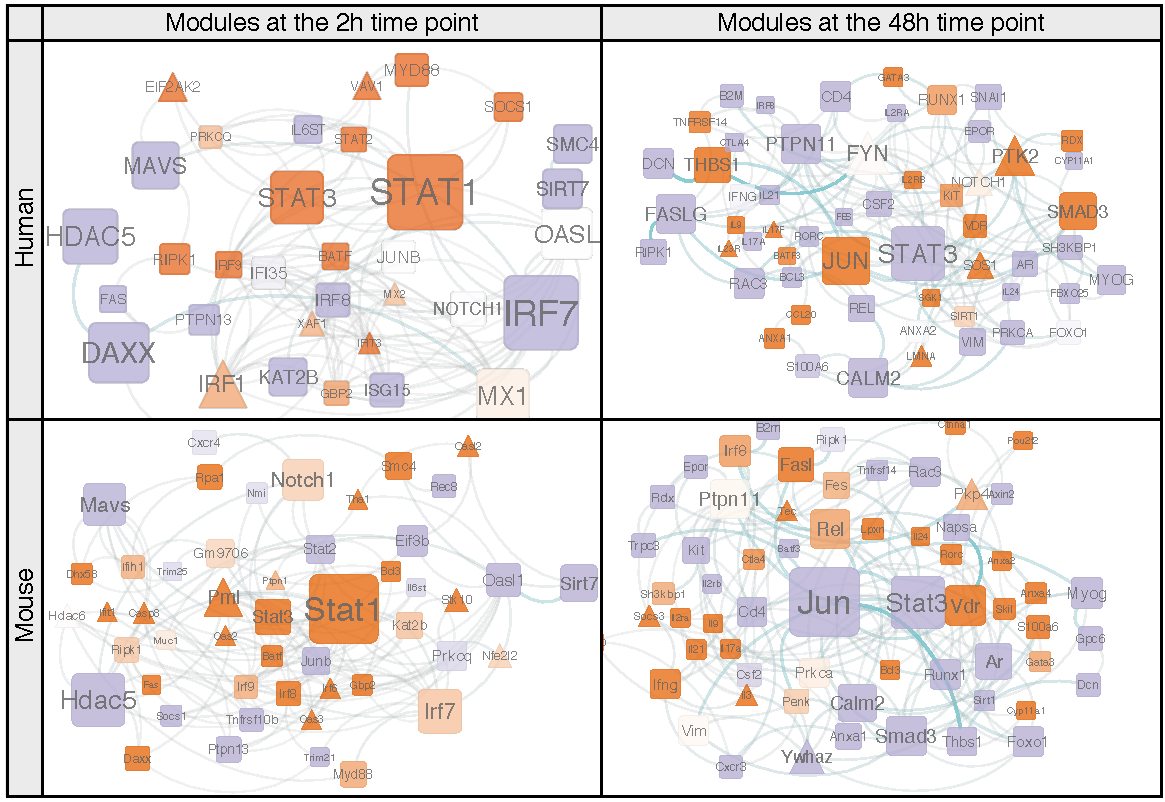
\includegraphics[width=\linewidth]{img/modules_panel.pdf}
  \caption[Conserved active Th17 differentiation modules in human and mouse at \unit{2}{h} and \unit{48}{h}]{\textbf{Conserved active Th17 differentiation modules in human and mouse at \unit{2}{h} and \unit{48}{h}.}
  We obtained node activity scores capturing the significance of differential gene expression between the Th17 and Th0 conditions in human and mouse using the BUM model with $\FDR = 0.1$.
  \xheinz{} uses these scores to search for conserved active modules in the STRING protein action network.
  The first row shows the human counterparts of the best scoring conserved modules for the \unit{2}{h} (left) and \unit{48}{h} (right) samples.
  The second row depicts the mouse counterparts.
  Rounded squares depict genes for which a homolog -- as defined by Ensembl -- is present in the counterpart, whereas triangles denote non-conserved genes.
  Node color gradually indicates activity scores.
  Orange: larger than $2$; white: between $-2$ and $2$; violet: smaller than $-2$.
  Node labels and sizes are proportional to betweenness centrality and edge width to
  edge-betweenness -- both centralities are with respect to the subnetwork module.
  Only nodes having a degree larger than $2$ (resp. $3$) are displayed for the \unit{2}{h} (resp. \unit{48}{h}) module.
  The full networks in tabular format are available on the accompanying website and in \cref{app:details}.
    }
\label{fig:panel_wht-xheinz_modules}
\end{figure}

\begin{figure}[p]
  \centering
  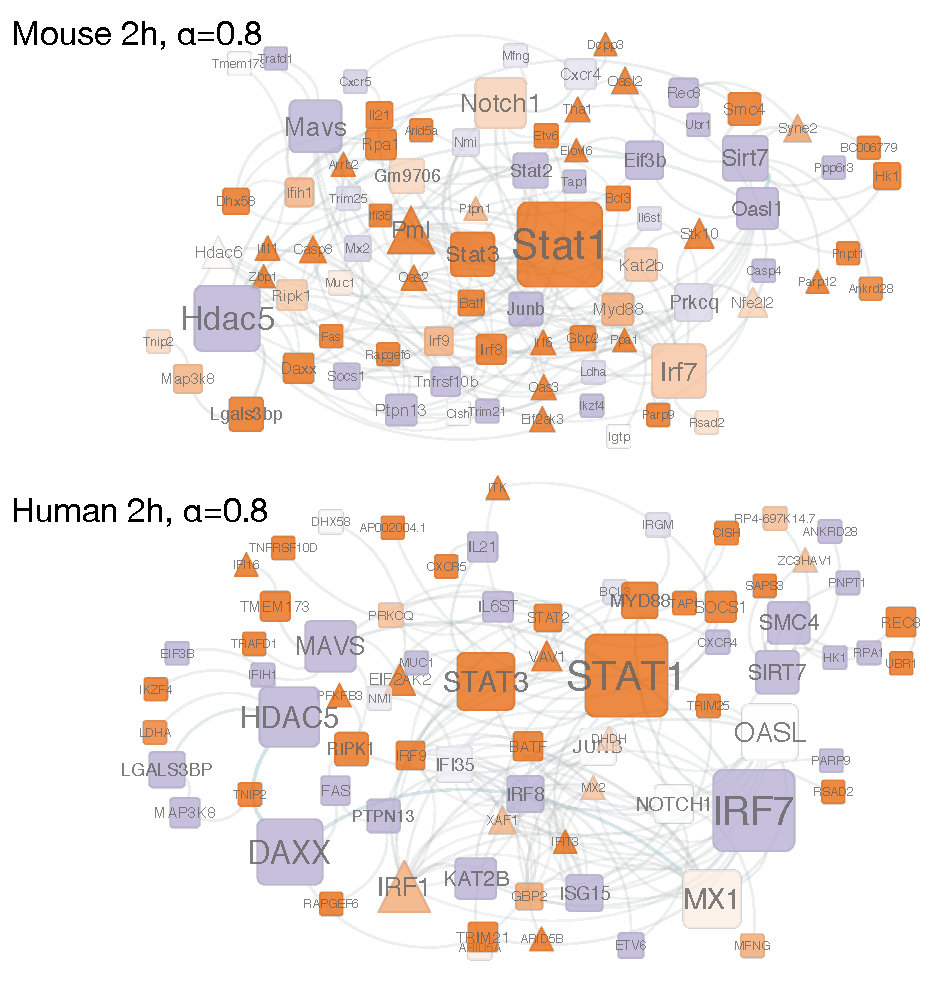
\includegraphics[width=\textwidth]{full_networks_2h.pdf}
  \caption{Full module at \unit{2}{h} for $\alpha = 0.8$ conservation ratio}
  \label{fig:full_1}
\end{figure}

\begin{figure}[p]
  \centering
  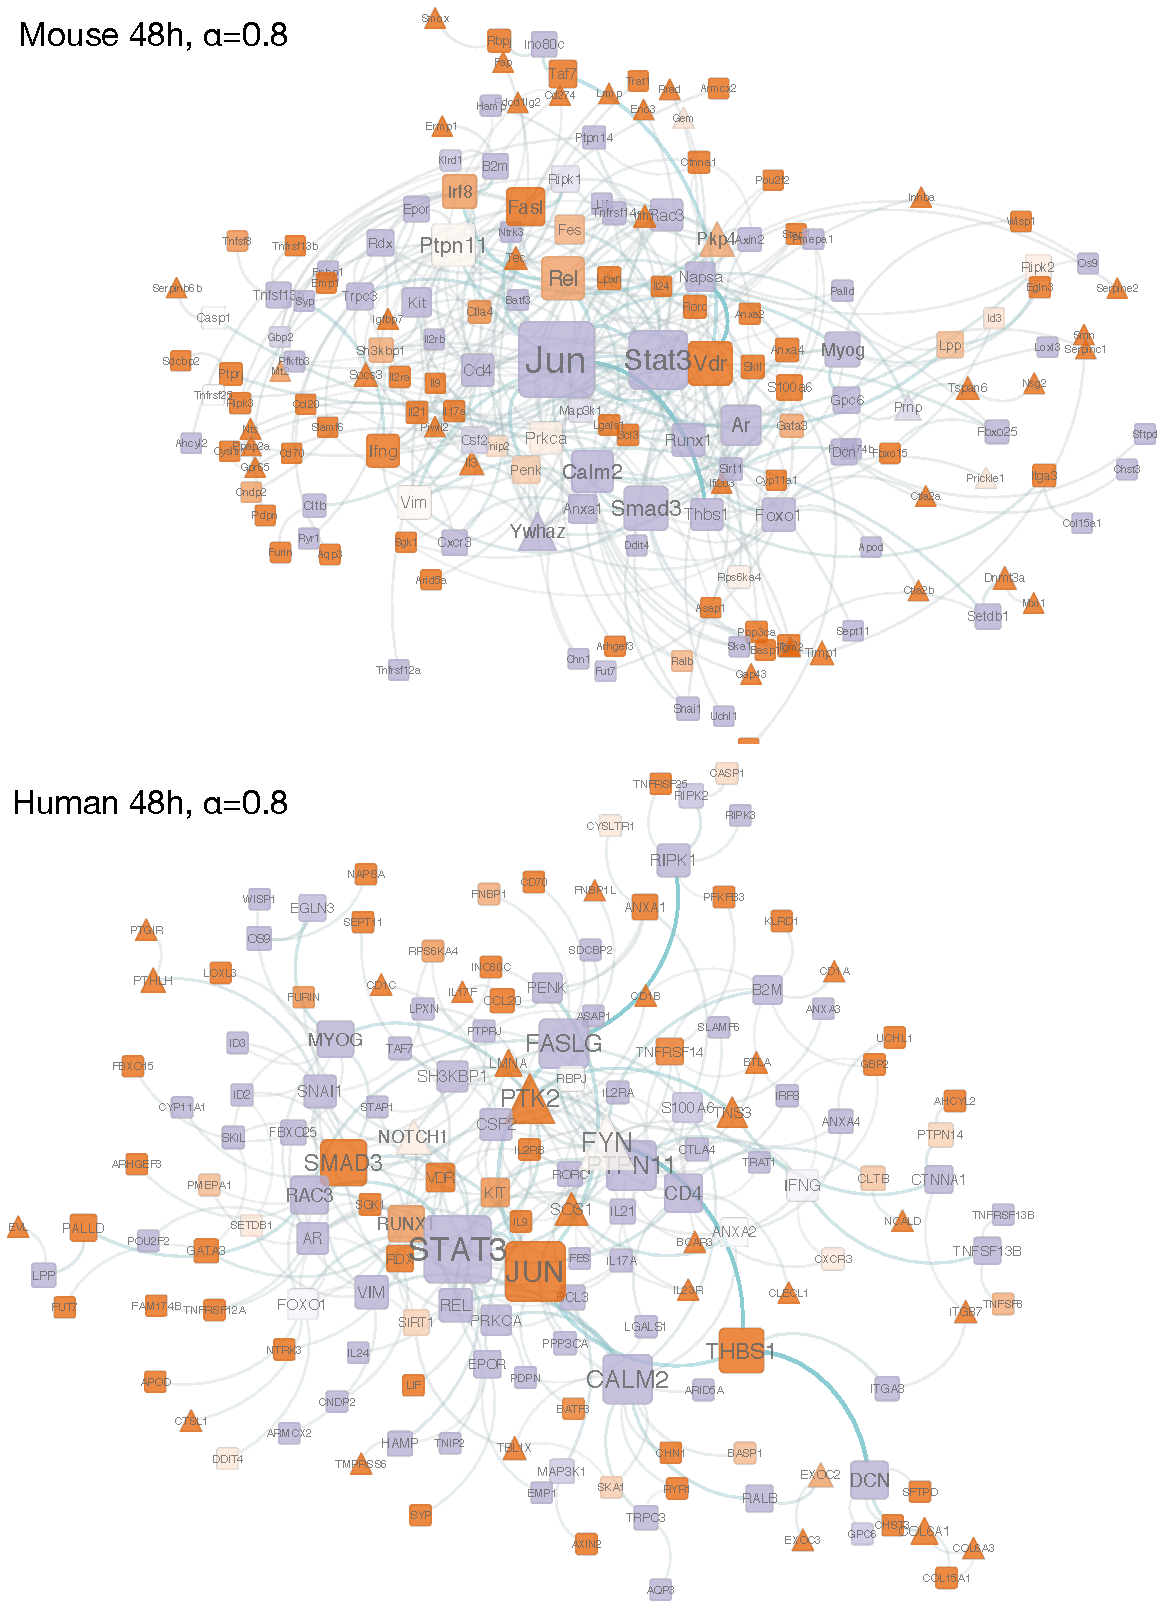
\includegraphics[width=\textwidth]{full_networks_48h.pdf}
  \caption{Full module at \unit{48}{h} for $\alpha = 0.8$ conservation ratio}
  \label{fig:full_2}
\end{figure}

% The parameter $\alpha$ represents as equilibrium between module's conservation
% and activity. We have evaluated if best conserved active modules show an
% increase in sequence similarity of selected proteins with an increase in
% $\alpha$. Indeed, sequence similarity is at the basis of most algorithms for
% identification of orthologous groups and in particular COGs. However, sequence
% similarity does not automatically imply function conservation. In particular,
% naive use of sequence similarity groups together dissimilar multi-domain proteins
% that share a common domain \citep{Smith:97}, and can be fooled by
% promiscuous domains \citep{Doolittle:95,Marcotte:99}. This was overcome
% in COGs construction by manual curation and indeed it is possible to have two
% orthologous genes with relatively low similarity (e.g., HERE THE LOWEST SCORE
% FOR COGS). Nevertheless, we observe that correcting for co-activity and
% co-conservation mostly preserves genes having high sequence similarity.

% TODO HERE SPECULATE??? We hypothesize here that high differential activity is
% mostly conserved between species for those genes that not only have similar
% domain architecture and function, but are highly similar in their sequences.

% subsection
% main_regulation_of_th17_differentiation_is_conserved_between_human_and_mouse
% (end)

\subsubsection{Comparison to \nexus{}}
\label{sec:Nexus}

We compare the \unit{48}{h} \xheinz{} modules (see \cref{fig:panel_wht-xheinz_modules,fig:full_1,fig:full_2}) with subnetworks computed by \nexus{} version 3 \parencite{deshpande2010scalable}.
In contrast to our exact approach, \nexus{} uses a heuristic technique to grow subnetworks from seed nodes simultaneously in two species in an iterative fashion.
Neighborhoods of the two current modules are determined using a depth-first search.
This search is restricted to only consider nodes that have a path to the seed node with a confidence larger than the user-specified parameter $\mathtt{dfscutoff}$.
The confidence of a path is defined as the product of the confidences of the edges comprising that path.
The modules are extended to include the most active pair of orthologous nodes in the neighborhoods -- where activity is defined as normalized log fold change and thus differs from the definition of activity used in \xheinz{}.
This whole procedure is repeated until either the cluster coefficient drops below the user-specified parameter $\mathtt{cc}$, or the average activity scores of one of the two modules drops below parameter $\mathtt{scorecutoff}$.

We ran \nexus{} with the default parameters $\mathtt{cc = 0.1,0.2}$, $\mathtt{scorecutoff=0.15}$ and $\mathtt{dfscutoff=0.3,0.8}$ for mouse and human respectively for all time points. \Cref{tab:nexus_all} gives the resulting modules sizes for human and mouse.

\begin{table}[h]
	\centering
	\makebox[0pt]{
	\scriptsize
	\tabcolsep=0.075cm
	\begin{tabular}{lp{7.4mm}p{7.4mm}p{7.4mm}p{7.4mm}p{7.4mm}p{7.4mm}p{7.4mm}p{7.4mm}p{7.4mm}p{7.4mm}p{7.4mm}p{7.4mm}p{7.4mm}p{7.4mm}p{7.4mm}lp{7.4mm}rp{7.4mm}}
	\hline
	solution & 1 & 2 & 3 & 4 & 5 & 6 & 7 & 8 & 9 & 10 & 11 & 12 & 13 & 14 & 15 & avg. & \#sols\\ \hline
	0.5h & 7 (6) & 4 (4) & 7 (6) & 3 (3) & & & & & & & & & & & & 5.25 (4.75) & 4\\
	1h & 15 (10) & 10 (9) & 12 (12) & 13 (13) & 7 (7) & 5 (5) & 15 (13) & 10 (11) & 9 (10) & 18 (16) & 25 (24) & 14 (14) & 6 (7) & 5 (5) & 6 (6) & 9.95 (9.58) & 19\\
	2h & 15 (17) & 6 (5) & 12 (10) & 12 (11) & 10 (10) & 13 (13) & 17 (15) & 12 (12) & 8 (9) & 5 (5) & 11 (12) & 19 (18) & 3 (3) & 9 (8) & 23 (21) & 10 (9.83) & 30\\
	4h & 6 (9) & 4 (4) & 6 (5) & 4 (4) & 4 (4) & 3 (3) & 7 (8) & 9 (10) & 4 (4) & 3 (3) & & & & & & 5 (5.40) & 10\\
	48h & 5 (5) & & & & & & & & & & & & & & & 5 (5) & 1\\
	\hline
	\end{tabular}
	}
	\caption[Modules calculated with \nexus{} for all time points]{\textbf{Modules calculated with \nexus{} for all time points.}
	Shown are the sizes in number of nodes of the first 15 representative solutions and the average sizes for the human subnetwork and for the mouse subnetwork in brackets.
	The last column lists the number of solutions for each time point.
	No solutions were obtained for time points \unit{24}{h} and \unit{72}{h}.
	}
	\label{tab:nexus_all}
\end{table}

\nexus{} finds 1 module for time point \unit{48}{h} which is shown in \cref{fig:nexus} for human (A) and mouse (B).
In total 5 genes are contained in the module, which are identical for human and mouse, but the number of edges differs.
Only one of the genes is significantly differentially expressed, CCL20, which has an absolute log fold change bigger than 1 and a BH FDR smaller than 0.1.
Since \nexus{} does not use p-values as an input, but log fold-changes which are normalized to activity values, the genes CCL20 and CXCR3 are considered as active nodes with a value above 0.15.
These genes show changes in expression, but only two of these changes are statistically significant.

The low number of active nodes points to a drawback in the \nexus{} algorithm: due to the locality of the greedy search strategy it may happen that the average activity of the subnetwork in construction keeps on degrading without reaching the next active node.
The effects of this issue can be seen, for example, in \cref{fig:nexus}, where CCL20 is the seed node and the majority of other neighboring nodes are not differentially expressed.
Furthermore, since the activity score of a single gene is just the log fold-change, and does not reflect both fold change and variability as a p-value, the neighboring nodes of the seed node in subnetwork \cref{fig:nexus} might merely originate from the noise in the data and represent nothing biologically relevant for the interpretation of the data.

\begin{figure}[h]
	\centering
	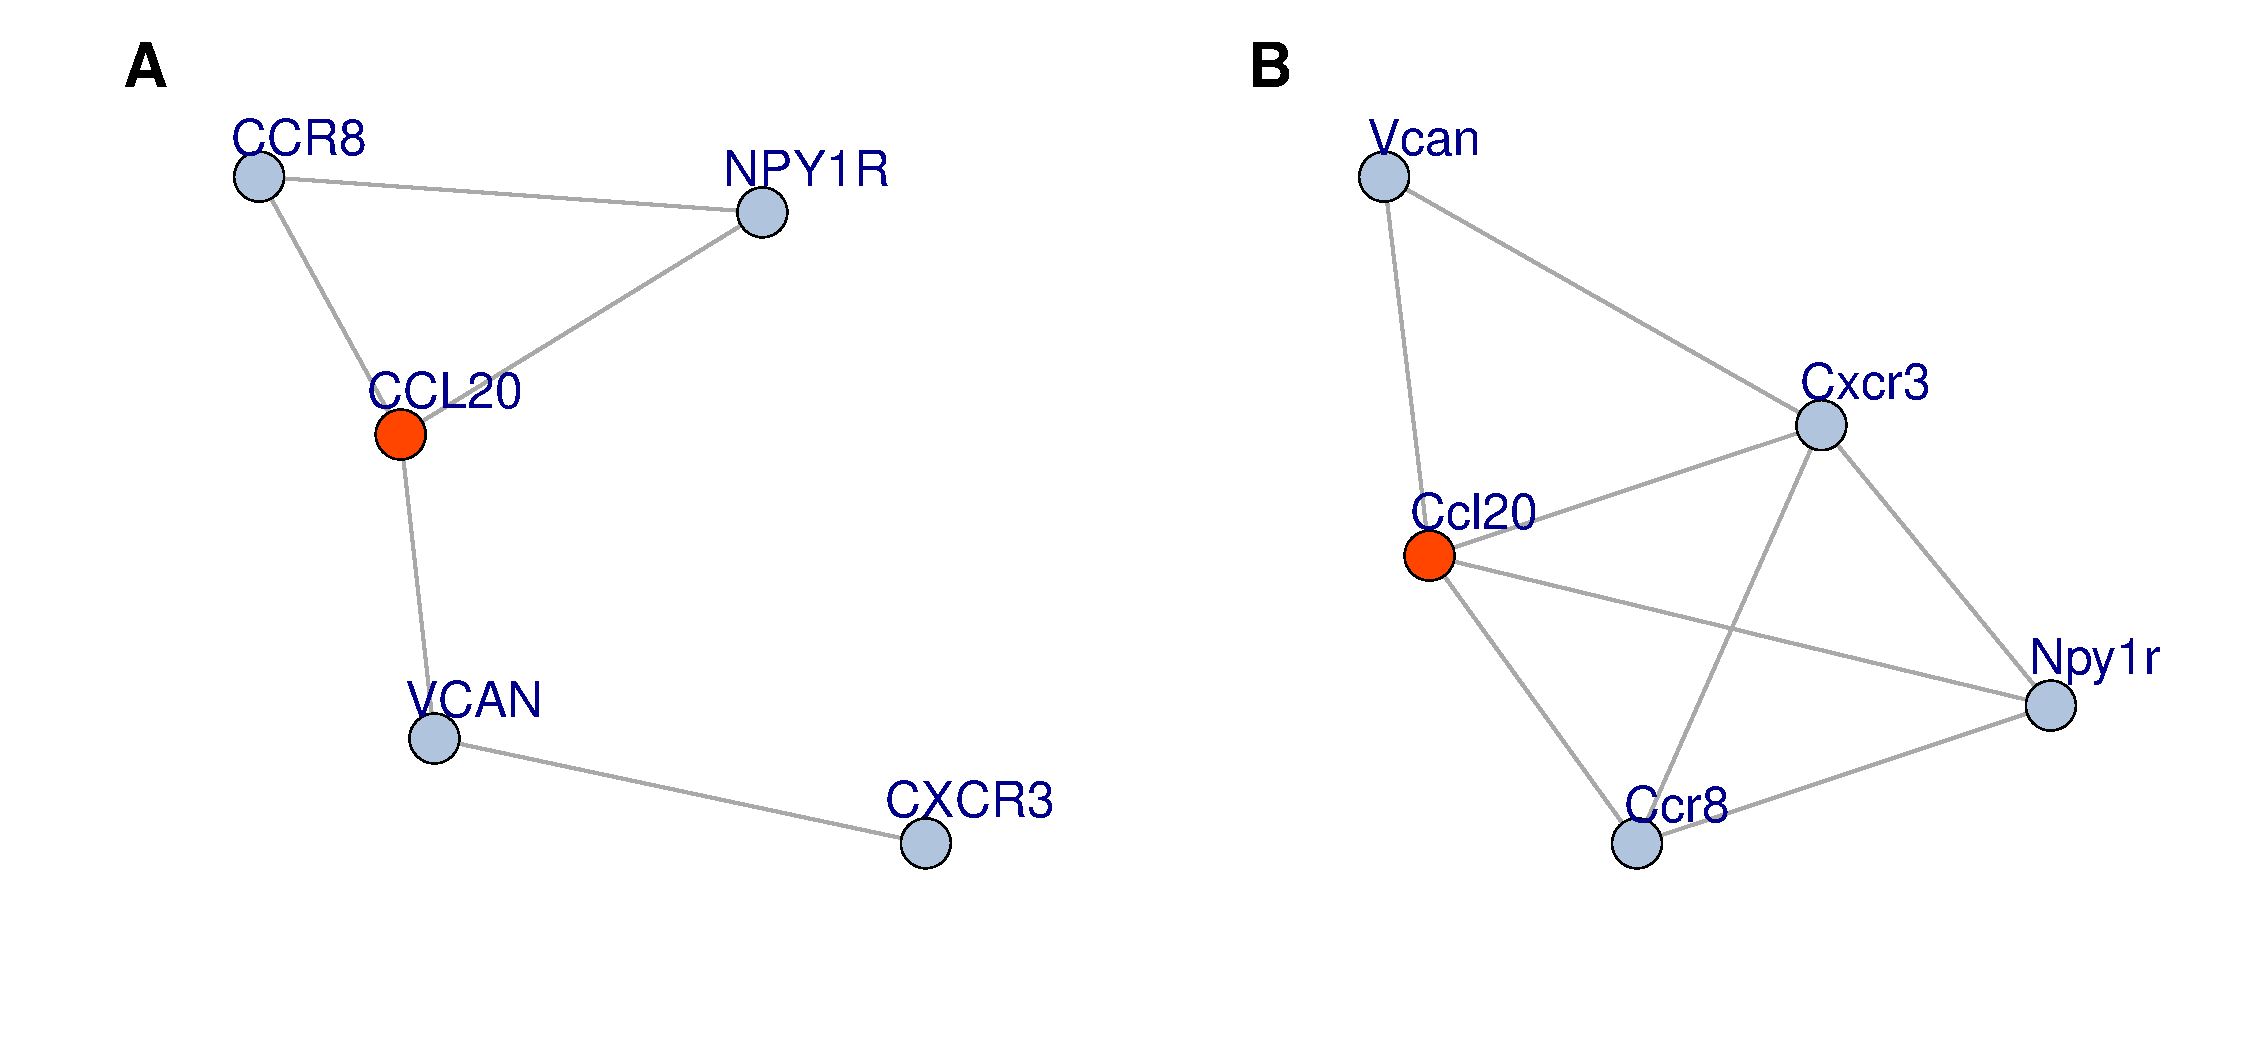
\includegraphics[width=\linewidth]{img/Nexus_module_A.pdf}
	\caption[\nexus{} modules for the time point 48 hours for human and mouse]{\textbf{\nexus{} modules for the time point 48 hours for human (A) and mouse (B).}
	Orange coloring indicates genes with significant differential expression (BH FDR $\leq 0.1$, $\absLOGFC \geq 1$).
	Here only one gene is significantly differentially expressed (CCL20).
	}
	\label{fig:nexus}
\end{figure}

\paragraph{}
Another consequence of the \nexus{} search strategy is that the module sizes are small (see \cref{tab:nexus_all}) and thus only give a limited view of the molecular mechanisms at play.
Theoretically, the parameter $\mathtt{dfscutoff}$ can be decreased to increase the module size.
Doing so, however, produces only slightly larger modules, but drastically increases the running time.
\Cref{tab:dfs} shows the \nexus{} solutions for time point \unit{48}{h} with different values for parameter \texttt{dfscutoff}.

\begin{table}[h]
	\caption[\nexus{} solutions for time point \unit{48}{h} with different values for parameter \texttt{dfscutoff}.]{\textbf{\nexus{} solutions for time point \unit{48}{h} with
    different values for parameter \texttt{dfscutoff}.} Shown are  the number of solutions, the average and maximum number of nodes and running times for the human network.}
\begin{center}
\tabcolsep=0.08cm
%\small
%%\color{red}
\begin{tabular}{lrrrrrrr}
\hline
dfscutoff & no.\ sols. & avg.\ size & max.\ size& CPU time [s] \\ \hline
0.1 & 2 & 5.00 & 5 & 176039.91\\
0.2 & 3 & 7.00 & 9 & 110282.61\\
0.3 & 5 & 6.60 & 9 & 77502.13\\
0.4 & 4 & 6.62 & 10 & 54972.92\\
0.5 & 6 & 5.58 & 9 & 35360.42\\
0.6 & 4 & 5.38 & 6 & 20538.4\\
0.7 & 3 & 5.33 & 6 & 11164.19\\
0.8 & 60 & 4.04 & 6 & 4639.59\\
0.9 & 0 & 0.00 & 0 & 1359.87\\ \hline
\end{tabular}
\end{center}
\label{tab:dfs}
\end{table}


Also note that changes in the clustering coefficient parameter $\mathtt{cc}$ only reduce the module size with increasing $\mathtt{cc}$.
\Cref{tab:cc} shows the \nexus{} solutions for time point \unit{48}{h} with different values for parameter \texttt{cc}.

\begin{table}[h]
	\caption[\nexus{} solutions for time point \unit{48}{h} with different values for parameter \texttt{cc}]{\textbf{\nexus{} solutions for time point \unit{48}{h} with
    different values for parameter \texttt{cc}.} Shown are  the number of solutions, the average and maximum number of nodes and running times for the human network.}
\begin{center}
\tabcolsep=0.08cm
%\small
%%\color{red}
\begin{tabular}{lrrrrrrr}
\hline
cc & no.\ sols. & avg.\ size & max.\ size& CPU time [s] \\ \hline
0.1 & 1 & 5 & 5 & 23367.68\\
0.2 & 1 & 5 & 5 & 23243.83\\
0.3 & 1 & 5 & 5 & 23903.09\\
0.4 & 1 & 5 & 5 & 24285.30\\
0.5 & 1 & 3 & 3 & 24318.78\\
0.6 & 1 & 3 & 3 & 24059.59\\
0.7 & 1 & 3 & 3 & 24518.68\\
0.8 & 1 & 3 & 3 & 24321.92\\
0.9 & 1 & 3 & 3 & 24246.56\\ \hline
\end{tabular}
\end{center}
\label{tab:cc}
\end{table}
%%}

\paragraph{}
Conservation in \nexus{} is enforced stringently by only allowing pairs of orthologous genes or genes that are only present in one of the networks to be included in the subnetworks (see \cref{fig:nexus}).
This is too restrictive if the underlying mechanisms in the two species differ.
For instance, for time point 48 hours and all but $\alpha=1$ values, \xheinz{} finds the non-conserved gene IL23R (BH FDR 3.52e-8, score 14.50, logFC 1.38) in human, which is involved in Th17 autocrine signaling \parencite{wei200721} but which is not differentially expressed in mouse.
\xheinz{} also finds JUNB, which at the 2 hour time point is up-regulated in human data (BH FDR 1e-2, score 0.02, logFC 1.3) and not detected as differentially expressed in the mouse data (BH FDR 0.48, score -4.01, logFC 0.65).
JUNB is a known partner of BATF with which it heterodimerizes preferentially during Th17 differentiation \parencite{schraml2009ap}, indicating its relevance.
Both important genes would have been missed by a more restrictive conservation setting.
Indeed, both \nexus{} and \xheinz{} at $\alpha = 1$ fail to find these genes showing that a more flexible view on conservation is required to adequately deal with transferability.

\section{Implementation and evaluation details}
	\subsection{Implementation}

	\xheinz{} is implemented in modern C++14 using the best practice patterns recently introduced by \textcite{meyers2014effective}, and makes use of the boost libraries and the LEMON graph library \parencite{dezsHo2011lemon}.
		CPLEX 12.6 is used as a black-box solver for our Mixed-Integer Linear Program formulation.
		The source code is publicly available in a git repository linked to from \mbox{\url{http://software.cwi.nl/xheinz}}.

		\paragraph{}
		Given two species, \xheinz{} takes as input:
		\begin{enumerate}
			\item a network for each of the species: $G_1$ and $G_2$,
			\item a mapping between the nodes of the two networks,
			\item scores associated to each of the nodes, \eg, derived from the p-value of the moderated t-test,
			\item the threshold value $\alpha$, and
			\item an optional time limit.
		\end{enumerate}

		\xheinz{} returns two node sets corresponding to a solution found within the time limit together with an upper bound on the optimal objective value.
		If the objective value equals this upper bound, the computed solution is provably optimal.

  \subsection{Data processing pipeline}
  The full pipeline, implemented using Snakemake, from data downloading to running xheinz, goes as follows:\pagebreak
  \begin{enumerate}
    \item Retrieve human and mouse ENSEMBL orthologs, STRING species specific network
    \item Retrieve human dataset from GEO (all time points, all conditions)
    \item Annotate human probes with ENSEMBL 
    \item Select human probes based on variance filter
    \item Perform linear modeling of the whole human dataset 
    \item Retrieve mouse dataset (all time points, all conditions)
    \item Annotate mouse probes with ENSEMBL 
    \item Select mouse probes based on variance filter
    \item Perform linear modeling of the whole mouse dataset 
    \item For each time point of interest: 
    \begin{enumerate}
      \item Call differentially expressed human genes by contrasting the Th17 with the Th0 condition $\Rightarrow$ p-value for each gene at this time point
      \item Call differentially expressed mouse genes by contrasting the Th17 with the Th0 condition $\Rightarrow$ p-value for each gene at this time point
      \item For an FDR threshold of 0.1, fit a BUM model for the human genes $\Rightarrow$ positive and negative scores for human genes
      \item For an FDR threshold of 0.1, fit a BUM model for the mouse genes $\Rightarrow$ positive and negative score for mouse genes 
      \item Rank normalize the mouse score based on the human scores $\Rightarrow$ update the scores of the mouse genes
      \item Map human and mouse genes to proteins on the STRING network
      \item For each value of interest for the conservation threshold $\alpha$:
      \begin{enumerate}
        \item Run xHeinz with the following inputs: 
        \begin{enumerate} 
          \item the human STRING network 
          \item the mouse STRING network
          \item the BUM scored human proteins
          \item the BUM scored mouse proteins
          \item the human and mouse orthologs
        \end{enumerate}
      \end{enumerate}
    \end{enumerate}
  \end{enumerate}

  \subsection{Significance of results}
  \label{app:significance}

  We computed empirical p-values to assess the significance of
  the obtained scores at \unit{2}{h} and \unit{48}{h}, for each value of
  $\alpha \in \{0.1, 0.2, \ldots, 1.0\}$, with the following two procedures:
  \begin{enumerate}
    \item \emph{Weights permutation:} We shuffled the node weights by generating random permutations of the activity scores of all genes.
    \item \emph{Topology permutation:} We repeated a million times the following operation: given two randomly selected edges A1--A2 and B1--B2, if the edges A1--B2 and B1--A2 are not present in the network we add them and remove the original edges, thus generating a random network with the same node weights and degree distribution.
  \end{enumerate}

  For each resulting permuted network we applied a modified version of xHeinz a
  fixed number of times (500 times for $\alpha = 0.8$, 100 times otherwise). This
  modified version allows to check whether the optimal score on the new random
  network would exceed the best score we found on the original network.

  To speed up these computations, we used the observation that solving a relaxed
  version of the conserved modules problem is sufficient, since we only need a
  sufficiently low upper bound (less than the score we obtained with unshuffled
  data) on the optimal values for those shuffled instances to make this decision.
  
  We therefore consider the following ILP for the shuffled instances:
  \allowdisplaybreaks
  \begin{alignat}{3}
   \label{eq:relaxed}\max\: & \sum_{v \in V_1 \cup V_2} w_v x_v \\
   \text{s.t.}\:\: & \eqref{eq:m_u}, \eqref{eq:m_v},
  \eqref{eq:b}, \eqref{eq:vars}
  \end{alignat}
  that is, we drop the connectivity constraints. Note that the objective
  value is an upper bound of the optimal score of the original problem
  since this new ILP is a relaxation of the original one. In
  addition, we can stop the branch-and-cut algorithm as soon as the
  upper bound on \eqref{eq:relaxed} is lower than the best found
  solution of the original ILP on the unshuffled data. These two
  observations help to speed up the significance computations tremendously.

  \Cref{tab:pval} shows the results of these runs, which we
  performed using a cumulative time limit of \unit{500}{h}. It can be seen that only
  at extreme values of $\alpha$ for the \unit{48}{h} time point the
  upper bound on \eqref{eq:relaxed} was not good enough to prove
  significance. This result was actually expected, since the original run was the only one
  with a very high gap ($33.36\%$) at the end of the allocated timelimit.

  Note that the p-values $\hat p$ that we demonstrate here are actually upper bounds to the
  underlying p-values $p$ that we would obtain without the relaxation to the ILP.

  For all other combinations, including the ones we chose to compute the Th17 modules
  and where we computed even more permutations, our procedure
  demonstrates that the signal in the real network is useful to obtain a
  statistically significant score.

  \begin{center}
  \begin{table}[h]
  \centering
  \tabcolsep=0.08cm
  {%\small
  \begin{tabular}{| c | c | c | c | c | c |}
  \hline
  Timepoint & $\alpha$ & FDR & $k$ & $k'$ & $\hat p$ \\ \hline
  \unit{2}{h}  & 0.1 & 0.1 & 100 & 0   & 0.0   \\
  \unit{2}{h}  & 0.2 & 0.1 & 100 & 0   & 0.0   \\
  \unit{2}{h}  & 0.3 & 0.1 & 100 & 0   & 0.0   \\
  \unit{2}{h}  & 0.4 & 0.1 & 100 & 0   & 0.0   \\
  \unit{2}{h}  & 0.5 & 0.1 & 100 & 0   & 0.0   \\
  \unit{2}{h}  & 0.6 & 0.1 & 100 & 0   & 0.0   \\
  \unit{2}{h}  & 0.7 & 0.1 & 100 & 0   & 0.0   \\
  \textbf{\unit{2}{h}}  & \textbf{0.8} & \textbf{0.1} & \textbf{500} & \textbf{0}   & \textbf{0.0}   \\
  \unit{2}{h}  & 0.9 & 0.1 & 100 & 0   & 0.0   \\
  \unit{2}{h}  & 1.0 & 0.1 & 100 & 0   & 0.0   \\ \hline
  \unit{48}{h} & 0.1 & 0.1 & 100 & 7   & \textbf{0.07}  \\
  \unit{48}{h} & 0.2 & 0.1 & 100 & 4   & \textbf{0.04}  \\
  \unit{48}{h} & 0.3 & 0.1 & 100 & 0   & 0.0   \\
  \unit{48}{h} & 0.4 & 0.1 & 100 & 0   & 0.0   \\
  \unit{48}{h} & 0.5 & 0.1 & 100 & 0   & 0.0   \\
  \unit{48}{h} & 0.6 & 0.1 & 100 & 0   & 0.0   \\
  \unit{48}{h} & 0.7 & 0.1 & 100 & 0   & 0.0   \\
  \textbf{\unit{48}{h}} & \textbf{0.8} & \textbf{0.1} & \textbf{500} & \textbf{0}   & \textbf{0.0}   \\
  \unit{48}{h} & 0.9 & 0.1 & 100 & 0   & 0.0   \\
  \unit{48}{h} & 1.0 & 0.1 & 100 & 100 & \textbf{1.0} \\
   \hline
  \end{tabular}}
  \qquad
  {%\small
  \begin{tabular}{| c | c | c | c | c | c |}
  \hline
  Timepoint & $\alpha$ & FDR & $k$ & $k'$ & $\hat p$ \\ \hline
  \unit{2}{h}  & 0.1 & 0.1 & 100 & 0   & 0.0   \\
  \unit{2}{h}  & 0.2 & 0.1 & 100 & 0   & 0.0   \\
  \unit{2}{h}  & 0.3 & 0.1 & 100 & 0   & 0.0   \\
  \unit{2}{h}  & 0.4 & 0.1 & 100 & 0   & 0.0   \\
  \unit{2}{h}  & 0.5 & 0.1 & 100 & 0   & 0.0   \\
  \unit{2}{h}  & 0.6 & 0.1 & 100 & 0   & 0.0   \\
  \unit{2}{h}  & 0.7 & 0.1 & 100 & 0   & 0.0   \\
  \textbf{\unit{2}{h}}  & \textbf{0.8} & \textbf{0.1} & \textbf{500} & \textbf{0}   & \textbf{0.0}   \\
  \unit{2}{h}  & 0.9 & 0.1 & 100 & 0   & 0.0   \\
  \unit{2}{h}  & 1.0 & 0.1 & 100 & 0   & 0.0   \\ \hline
  \unit{48}{h} & 0.1 & 0.1 & 100 & 7   & 0.0   \\
  \unit{48}{h} & 0.2 & 0.1 & 100 & 4   & 0.0   \\
  \unit{48}{h} & 0.3 & 0.1 & 100 & 0   & 0.0   \\
  \unit{48}{h} & 0.4 & 0.1 & 100 & 0   & 0.0   \\
  \unit{48}{h} & 0.5 & 0.1 & 100 & 0   & 0.0   \\
  \unit{48}{h} & 0.6 & 0.1 & 100 & 0   & 0.0   \\
  \unit{48}{h} & 0.7 & 0.1 & 100 & 0   & 0.0   \\
  \textbf{\unit{48}{h}} & \textbf{0.8} & \textbf{0.1} & \textbf{500} & \textbf{0}   & \textbf{0.0}   \\
  \unit{48}{h} & 0.9 & 0.1 & 100 & 0   & 0.0   \\
  \unit{48}{h} & 1.0 & 0.1 & 100 & 20  & \textbf{0.2} \\
   \hline
  \end{tabular}}
  \caption[Results of significance experiments]{Results of significance experiments. For $\alpha \in \{0.1, 0.2,
  	\ldots, 1.0\}$ at time points \unit{2}{h} and \unit{48}{h} we computed upper
  	bounds on $k$ instances with permuted scores using the procedures described
  	above (weights permutation on the left, topology permutation on the right).
  	In $k'$ of these cases, %after a cumulative time limit of \unit{500}{h}, the
  	resulting upper bound was not lower than the score of the best found
  	conserved active module on the original network, resulting in a p-value $p
  \leq \hat p = k'/k$. Values at the threshold $\alpha = 0.8$ we used to compute
  the Th17 modules and non-zero p-values are highlighted.}
  \label{tab:pval}
  \end{table}
  \end{center}

  \subsection{Robustness of modules for varying $\alpha$}

  Given two modules $V_1' \subseteq V_1$ and $V_2' \subseteq V_2$, the
  Jaccard index is defined as $(V_1' \cap V_2')/(V_1' \cup
    V_2')$. Fig.~\ref{fig:jaccard_alpha} shows for each time point the
  Jaccard index for all pairs of conservation ratios. For consecutive
  values of $\alpha$ we can see that the module contents do not change
  much.

  Fig.~\ref{fig:focus_plot} shows the human gene module contents for time
  point \unit{2}{h} for varying values of $\alpha$, one gene per
  line. Genes in the left panel (FALSE) are negatively scored, that is,
  they are not differentially expressed at an FDR of 0.1. Genes in the
  right panel (TRUE) have a positive score. Squares represent conserved genes,
  whereas triangles represent non-conserved genes. An \xheinz module
  solution is thus the set of genes marked with a square or
  triangle at a given value of $\alpha$. The coloring is as follows:
  \begin{itemize}
  \item Genes that are selected at all values of $\alpha$ or
    are coloured red. These are the core genes. 
  \item Genes that are selected at $\alpha=0$ (no conservation)
    but not at $\alpha = 1$ are green. 
  \item Genes that are selected by $\alpha=1$
    (strict conservation) but not at $\alpha=0$ are turquoise. 
  \item Genes that can only be picked by \xheinz (intermediate $\alpha$ values)
    are orchid.
  \end{itemize}

  This figure shows that a large fraction of genes
  only occur in an intermediate $\alpha$ regime (orchid
  color). Furthermore, the module content smoothly changes as $\alpha$
  varies, which illustrates the robustness of the approach. \xheinz thus
  allows the investigator to make an informed choice on the conservation
  of genes in the modules, which is not possible with methods assuming
  no or strict conservation.

  \begin{figure}[b]
    \centering
    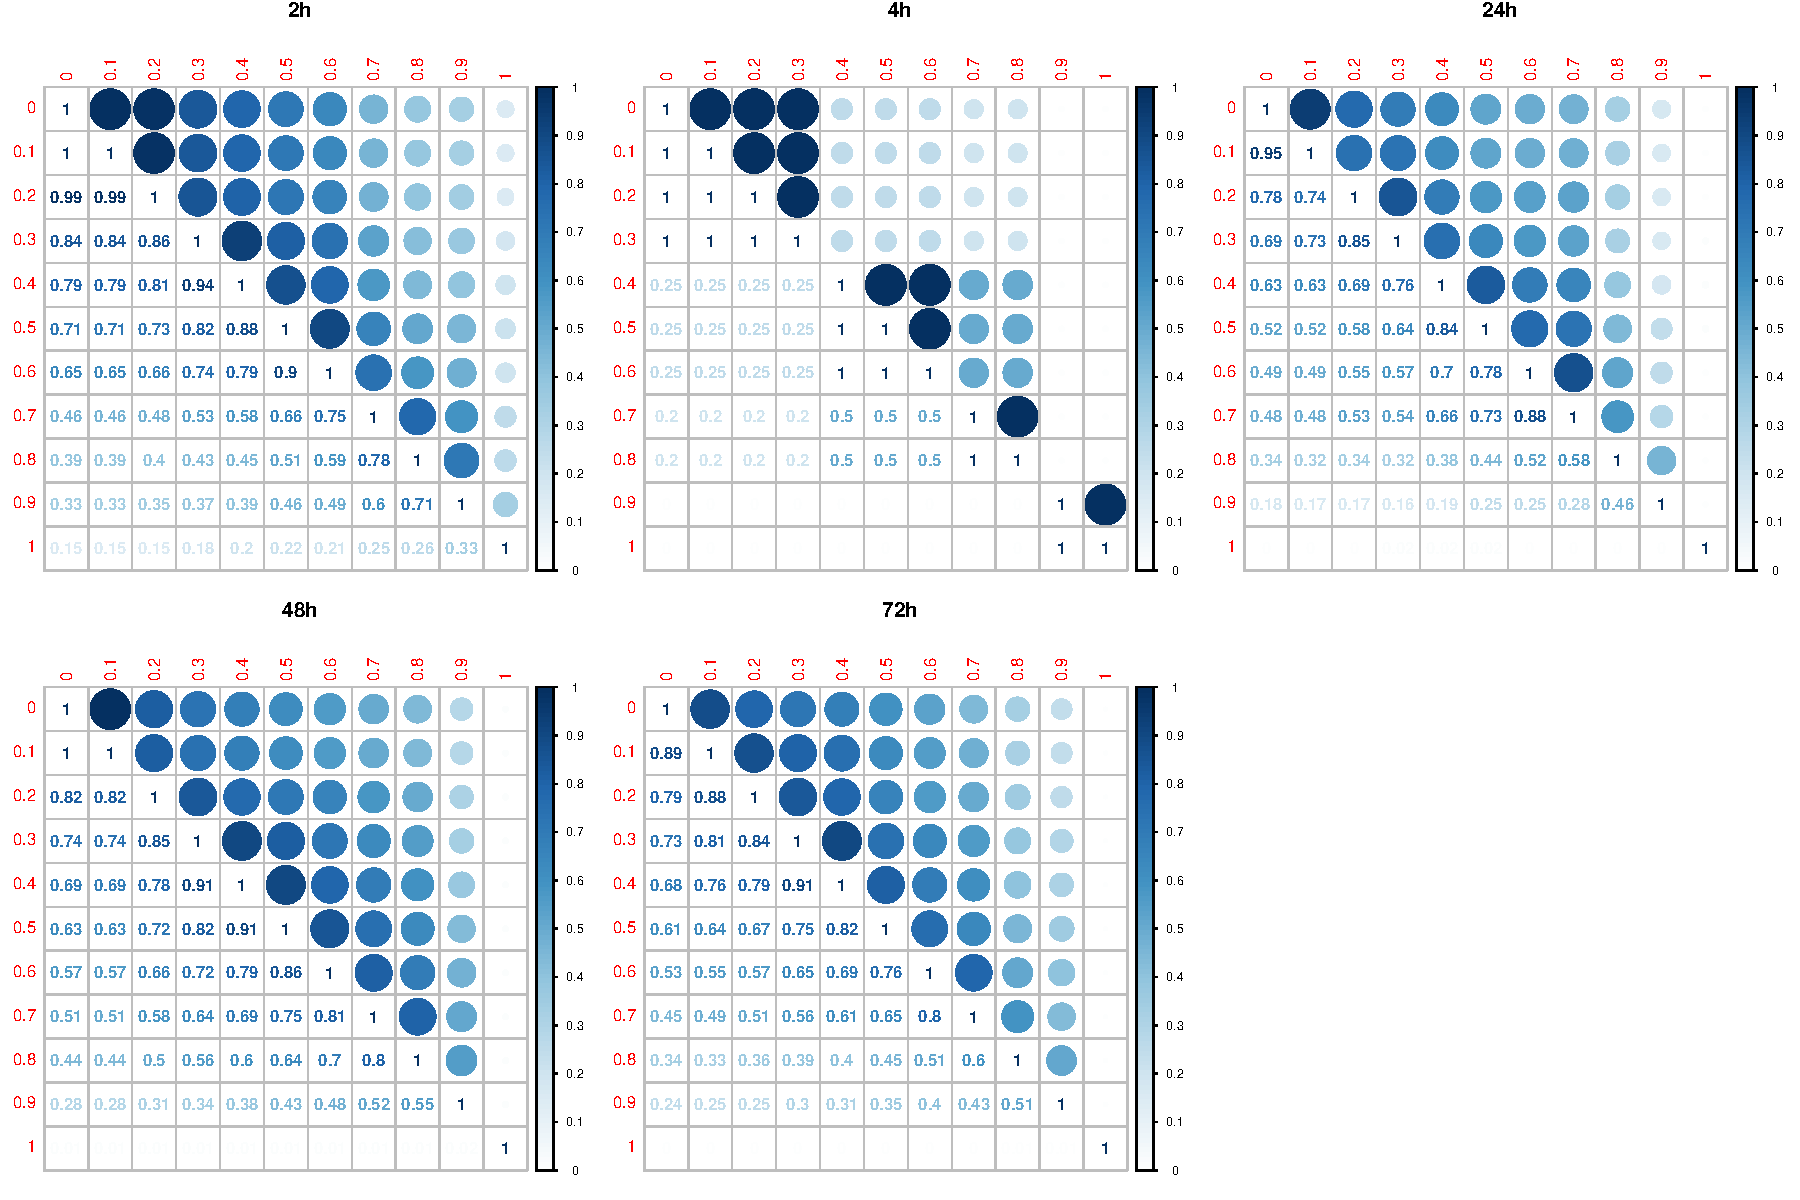
\includegraphics[width=1\linewidth]{jaccard_corrplot_numbers_v2.pdf}
    \caption{Jaccard index evolution over changes of $\alpha$}
    \label{fig:jaccard_alpha}
  \end{figure}

  \begin{figure}[p]
    \centering
    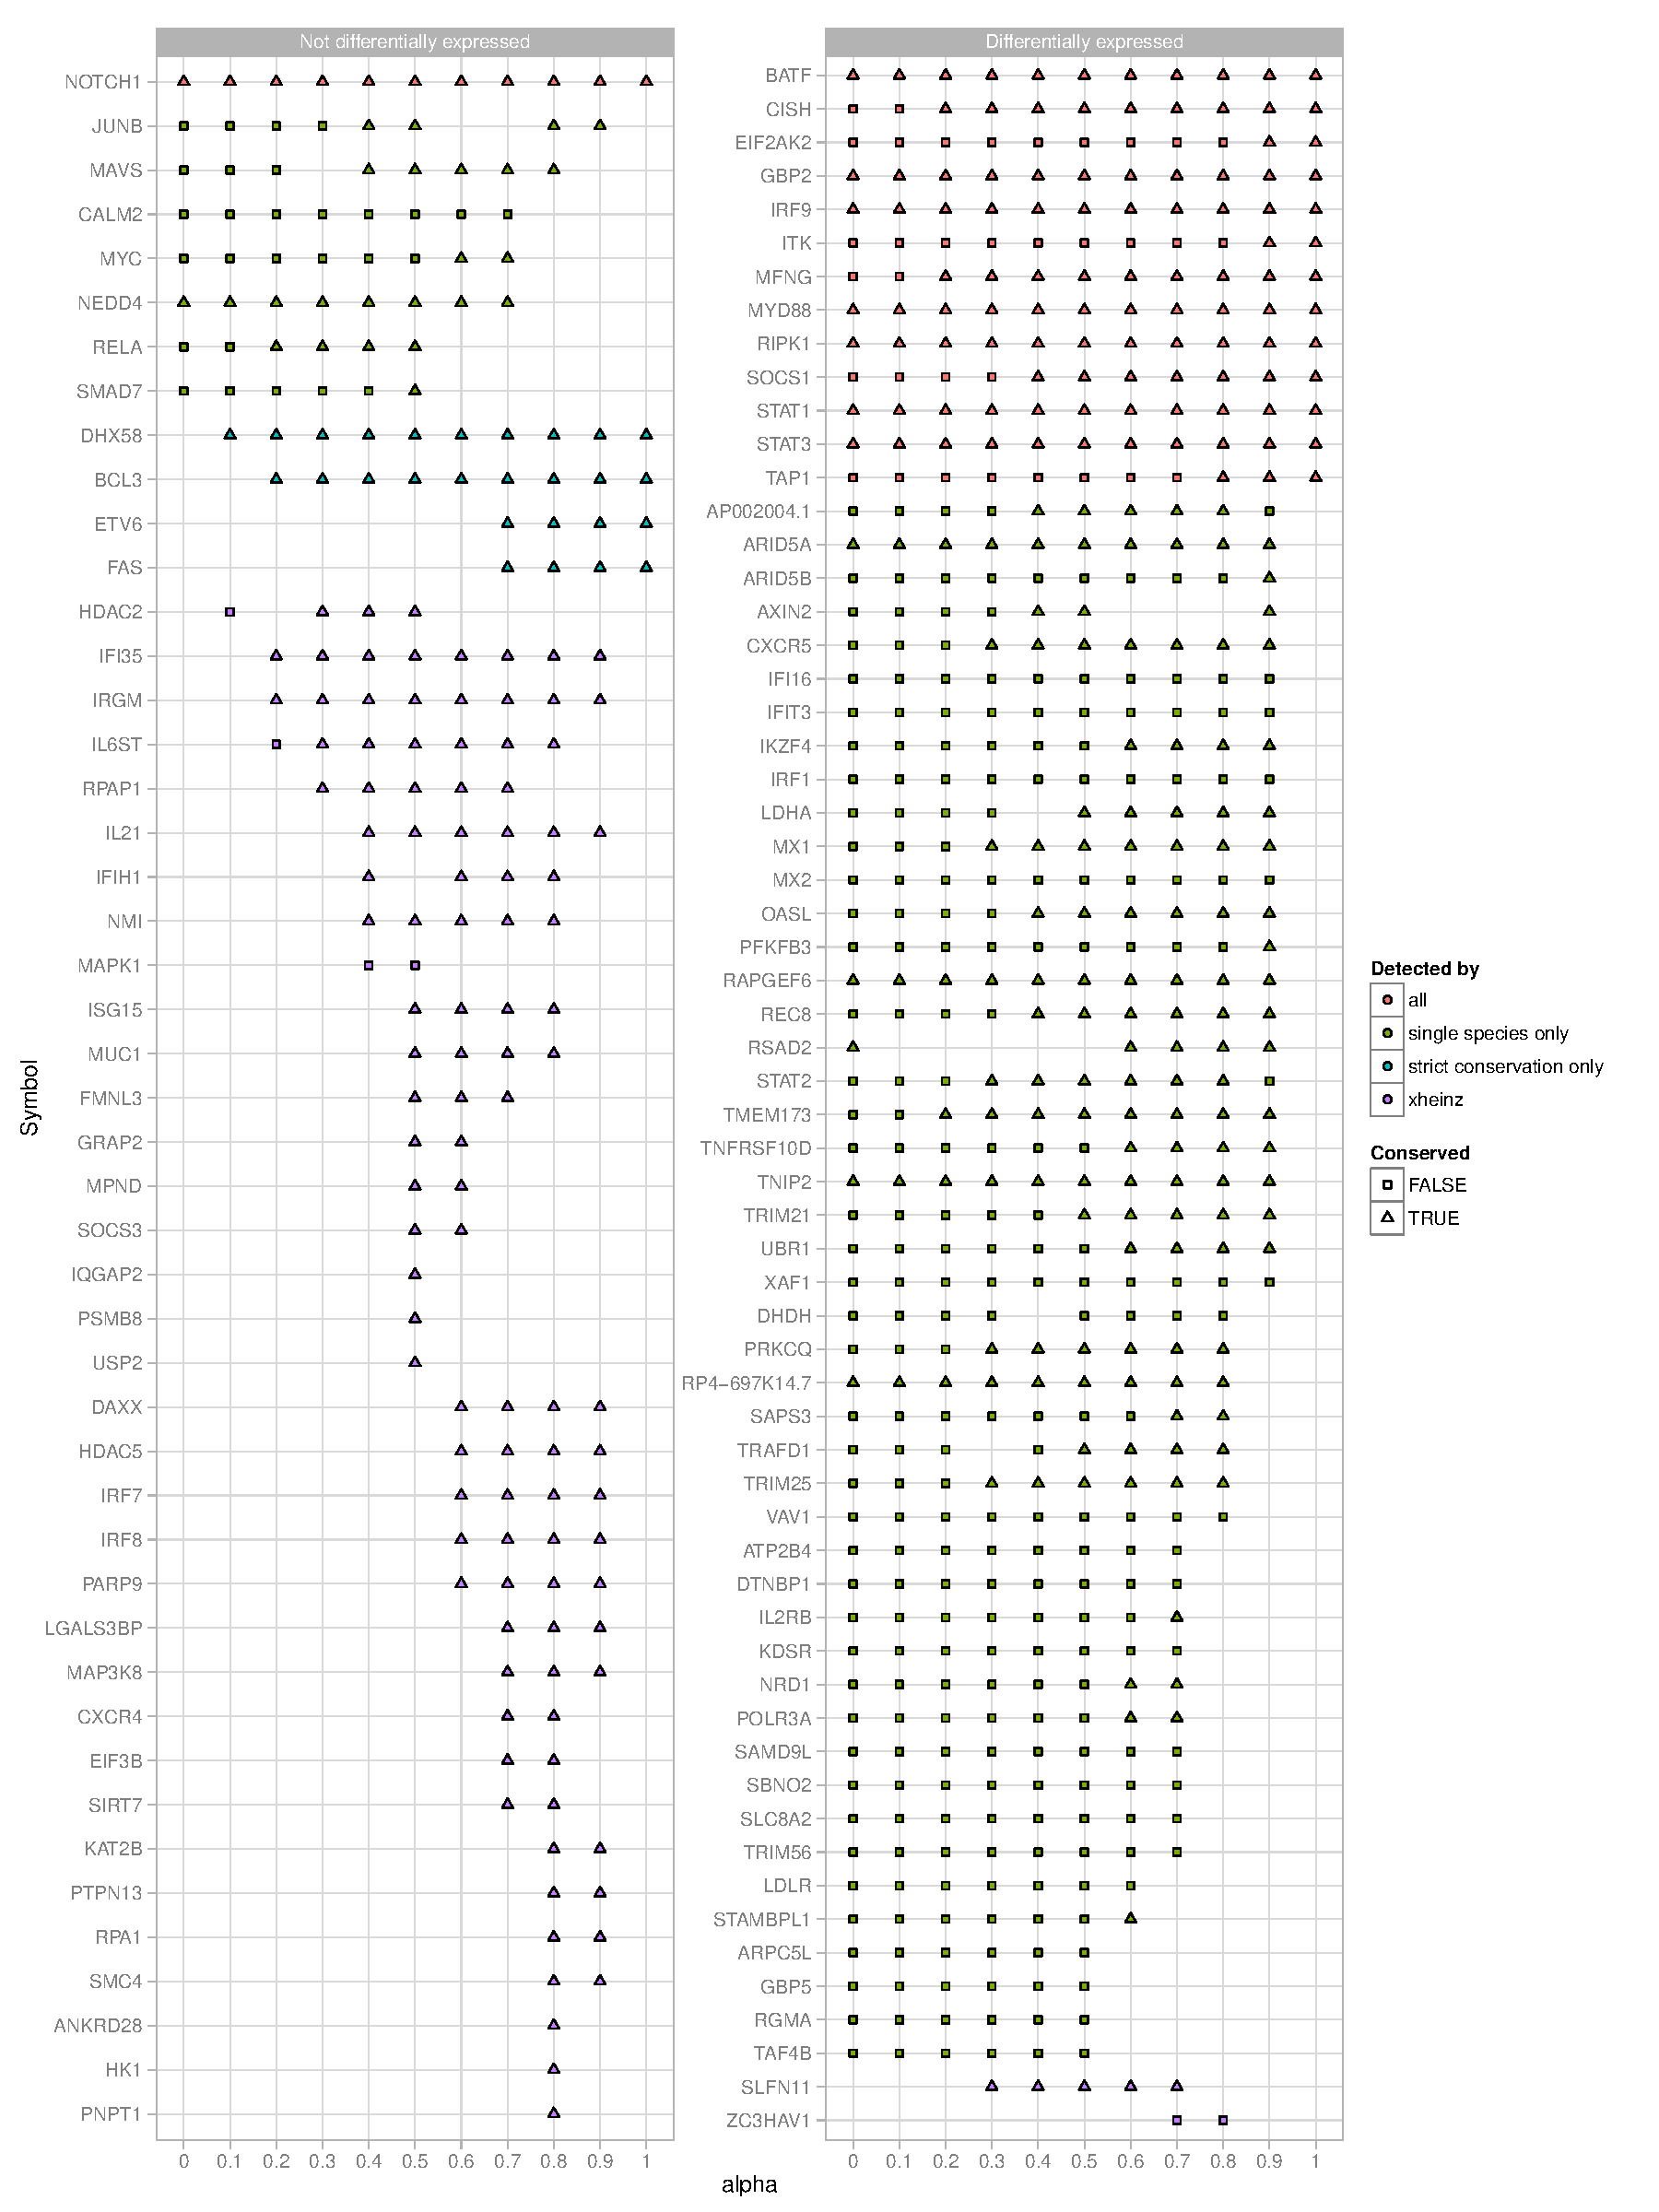
\includegraphics[width=1.2\linewidth]{focus_plot_2h_v2.pdf}
    \caption{Human module contents of the \unit{2}{h} time point with varying $\alpha$}
    \label{fig:focus_plot}
  \end{figure}

\section{Discussion}
\label{sec:xdisc}

We presented a module discovery method that simultaneously searches across two species for interesting gene sets.
A key feature of the gene sets that we extract is the guaranteed lower bound on the number of conserved genes that they contain.
This user defined lower bound, $\alpha \in [0, 1]$, provides a flexible conservation requirement between the two species, which allows for the discovery of conserved modules, including genes that would be missed with a stringent conservation requirement.%\footnote{Note that in the case of distantly-related species, a smaller $\alpha$ value may be more appropriate, which is a setup our model can be aptly applied to.}.
%In doing so, we thus contribute to the formalization of the notion of conserved active modules.

We have translated our model into an integer linear programming formulation and have devised and implemented an exact branch-and-cut algorithm that computes provably optimal or near-optimal conserved active modules in our model.

\paragraph{}
As a validation of our approach, our computational experiments for understanding the mechanisms underlying Th17 T cell differentiation in both mouse and human demonstrate that the flexibility in the definition of conservation is crucial for the computation of meaningful conserved active modules.
We have found two conserved Th17 modules at time points \unit{2}{h} ($\alpha = 0.8$) and \unit{48}{h} ($\alpha=0.8$) that thoroughly encompass the biphasic Th17 differentiation process.
This result can not be revealed by requiring full conservation ($\alpha = 1$) or by independent modules without requiring conservation ($\alpha = 0$).
Likewise, \nexus{}, an alternative approach based on a stringent conservation model, is not able to capture the key regulatory program of the differentiation process.

\paragraph{}
A key characteristics of our model is its flexibility.
This allows its extension to multiple species and time points, which we will address in future work.
In this case, however, realistic instances will be harder to compute to optimality.
Indeed, the number of interactions between multiple species or time points increase at least quadratically the number of both ILP variables and constraints.
It would requires the development of powerful algorithm engineering techniques.
Interestingly, the complexity of our branch-and-cut modelization of connectivity remains linear on the number of graphs involved.

%\paragraph{}
%It could be argued that gene conservation alone does not suffice to guarantee transferability.
%Indeed, recent studies in network alignment showed that biobjective models that look for both gene and interaction conservations tend to discover slightly different structures between species.
%
%However, since we deliberately opted for a constraint based representation of the conservation ratio\footnote{Instead of the more natural but problematic option of having the ratio as a free parameter to optimize for through the objective function.}, the model that we present in \ref{sec:mip} can be easily extended.
%Even though we specifically used a solver technique that does not model edges in the two graphs for performance reasons, there exists state of the art techniques that explicitly represent the edges, and that solve the \mwcs{} problem with competitive running times still (see chapter \emph{state of the art}).
%Using an explicit representation of the edges would allow for a very easy extension of our model.
%The interaction conservations would have to be explicitly represented in the inputs, for example with another bipartite graph linking edges in both graphs, and a conservation ratio constraint, similar to the one for genes, would be added to the integer model.
%
%Second, even though the mathematical model and the integer program are easy to modify, we decided to favor speed of execution in our current implementation.
%Indeed, the quality of most protein-protein interaction networks available is difficult to attest.
%Most of these networks are constructed using cross-species inferences, literature mining, and increasingly advanced techniques to statistically deduce protein interactions.
%We have found that filtering these networks for only the experimentally verified interactions results in most case in very sparse networks, which makes difficult any cross-species reasoning.

\paragraph{}
We presented a general model and its MIP program to solve any instance of the cross-species module discovery problem.
An extensive complexity analysis of the problem is presented in \cref{chap:hard}, where we show that some instances can be solved in polynomial time with specific algorithms.
